\documentclass{article}
\usepackage[english]{babel}
% Import the specific settings for the template
% Notes: math_settings.tex must be imported before graphics_settings.tex since cleveref must be loaded after amsmath
%        colors_settings.tex must be imported before custom_snippets.tex since the colors must be defined before the custom_snippets
\usepackage[table]{xcolor}
\definecolor{defcolor}{RGB}{213, 117, 3} 
\definecolor{thmcolor}{RGB}{11, 99, 7}    
\definecolor{excolor}{RGB}{137, 136, 136}     
\definecolor{exercisecolor}{RGB}{137, 136, 136} 
\definecolor{notecolor}{RGB}{7, 94, 99}   

\definecolor{codekeyword}{RGB}{18, 137, 172}
\definecolor{codestring}{RGB}{225, 133, 0}
\definecolor{codecomment}{RGB}{132, 130, 127}
\usepackage{amsmath}
\usepackage{amssymb}
\usepackage{amsthm}
\usepackage{mathtools}
\usepackage{dsfont} %to use the unitary symbol \mathds{1}
\DeclareMathAlphabet{\mathams}{U}{msb}{m}{n}
\newcommand{\E}{\mathams{E}}
\DeclareMathOperator*{\argmax}{arg\,max}
\DeclareMathOperator*{\argmin}{arg\,min}
\newcommand{\pd}[2]{\frac{\partial #1}{\partial #2}}
\newcommand{\dern}[3]{\frac{d^{#3} #1}{d #2^{#3}}}
\newcommand*\Laplace{\mathop{}\!\mathbin\bigtriangleup}
\newcommand{\Usvd}{
    \begin{bmatrix}
       | & | & & | \\
       u_1 & u_2 & \cdots & u_n \\
       | & | & & |
    \end{bmatrix}
}
\newcommand{\Uhatsvd}{
    \begin{bmatrix}
       | & | & & | \\
       u_1 & u_2 & \cdots & u_m \\
       | & | & & |
    \end{bmatrix}
}
\newcommand{\Vsvd}{
    \begin{bmatrix}
       | & | & & | \\
       v_1 & v_2 & \cdots & v_m \\
       | & | & & |
    \end{bmatrix}
}
\newcommand{\VTsvd}{
    \begin{bmatrix}
        - & v_1^T &- \\
        - & v_2^T &- \\
        & \vdots & \\
        - & v_m^T &- 
    \end{bmatrix}
}
\newcommand{\Ssvd}{\begin{bmatrix}
       s_1 & 0 & \cdots & 0 \\
       0 & s_2 & \cdots & 0 \\
       \vdots & \vdots & \ddots & \vdots \\
       0 & 0 & \cdots & s_m\\
       0 & 0 & \cdots & 0\\
       \vdots & \vdots & \ddots & \vdots \\
       0 & 0 & \cdots & 0
    \end{bmatrix}
}
\newcommand{\Shatsvd}{\begin{bmatrix}
       s_1 & 0 & \cdots & 0 \\
       0 & s_2 & \cdots & 0 \\
       \vdots & \vdots & \ddots & \vdots \\
       0 & 0 & \cdots & s_m
    \end{bmatrix}
}
\newcommand{\pseudoinv}[1]{#1^{\dagger}}
\usepackage{geometry}
\geometry{%
    left=4cm,%
    right=4cm,%
    top=3.5cm,%
    bottom=3cm,%
    bindingoffset=0cm,
}

\usepackage[colorlinks=true,allcolors=blue]{hyperref}
\usepackage[english,nameinlink]{cleveref}
\usepackage{cleveref}
\Crefname{table}{Table}{Tables}
\usepackage{multirow}
\usepackage{wrapfig}
\usepackage{float}
\usepackage{graphicx}
\usepackage{colortbl}
\newcommand{\HRule}[1]{\rule{\linewidth}{#1}}
\usepackage{tikz}
\usetikzlibrary{calc}
\usetikzlibrary{angles}
\usetikzlibrary{quotes}
\usetikzlibrary{arrows.meta}
\usepackage{caption}
\usepackage{subcaption}
\usepackage{adjustbox}
\usepackage[many]{tcolorbox}
\tcbset{
    colframe=magenta,
    colback=magenta!12!white,
    boxed title style={colback=magenta},
    breakable,
    enhanced,
    sharp corners,
    boxsep=1pt,
    attach boxed title to top left={yshift=-\tcboxedtitleheight,  yshifttext=-.75\baselineskip},
    boxed title style={boxsep=1pt,sharp corners},
    fonttitle=\bfseries\sffamily,
    drop lifted shadow
}

\newtcolorbox[auto counter,number format=\arabic]{definition}[1][]{
    title={Definition~\thetcbcounter},
    colframe=defcolor,
    colback=defcolor!0!white,
    boxed title style={colback=defcolor!80!white},
    overlay unbroken and first={
        \node[below right, font=\small, color=defcolor, text width=.8\linewidth] at (title.north east) {#1};
    }
}

\newtcolorbox[auto counter,number format=\arabic]{theorem}[1][]{
    title={Theorem~\thetcbcounter},
    colframe=thmcolor,
    colback=thmcolor!0!white,
    fontupper=\itshape,
    boxed title style={colback=thmcolor!80!white},
    overlay unbroken and first={
        \node[below right, font=\small, color=thmcolor, text width=.8\linewidth] at (title.north east) {#1};
    }
}

\newtcolorbox[auto counter,number format=\arabic]{example}[1][]{
    title={Example~\thetcbcounter},
    colframe=excolor,
    colback=excolor!0!white,
    boxed title style={colback=excolor!80!white},
    overlay unbroken and first={
        \node[below right, font=\small, color=excolor!80!white, text width=.8\linewidth] at (title.north east) {#1};
    }
}

\newtcolorbox[auto counter,number format=\arabic]{exercise}[1][]{
    title={Exercise~\thetcbcounter},
    colframe=exercisecolor,
    colback=exercisecolor!0!white,
    boxed title style={colback=exercisecolor!80!white},
    overlay unbroken and first={
        \node[below right, font=\small, color=exercisecolor, text width=.8\linewidth] at (title.north east) {#1};
    }
}

\newtcolorbox[auto counter,number format=\arabic]{note}[1][]{
    title={Note~\thetcbcounter},
    colframe=notecolor,
    colback=notecolor!0!white,
    boxed title style={colback=notecolor!80!white},
    overlay unbroken and first={
        \node[below right, font=\small, color=notecolor, text width=.8\linewidth] at (title.north east) {#1};
    }
}

\usepackage{listings}
\lstnewenvironment{python}[1][]{
    \lstset{
        language=Python,
        basicstyle=\small\ttfamily,
        numbers=left,
        numberstyle=\tiny\color{gray},
        keywordstyle=\color{codekeyword},
        stringstyle=\color{codestring},
        commentstyle=\color{codecomment},
        morekeywords={True, False, append, extend, insert, remove, pop, clear, index, count, sort, reverse},
        breaklines=true,
        frame=single,
        framesep=3pt,
        frameround=tttt,
        backgroundcolor=\color{gray!10},
        rulecolor=\color{black!30},
        tabsize=4,
        columns=flexible,
        captionpos=b,
        title=#1,
        literate={\ }{{\space}}1
    }
}{}
% Your additional packages and settings go here
\title{ \normalsize \textsc{}
		\\ [2.0cm]
		\HRule{1.5pt} \\
		\LARGE \textbf{{A kernel methods/DL pipeline for the FashionMNIST dataset} 
		\HRule{2.0pt} \\ [0.6cm] \Large{Challenge 1 (Advanced Deep and Kernel Methods)} \vspace*{10\baselineskip}}
		}
\author{MSc's degree in Data Science and Artificial Intelligence (DSAI) \\[0.3cm]
        Fantuzzi Giulio [SM3800012]}
\date{Academic year 2024-2025}

\begin{document}
    %\maketitle
    %\newpage
    \begin{titlepage}
        \begin{center}
            \begin{figure}[ht]
                \centering
                
\includegraphics[width=\textwidth]{images/multiple_logo.png}
            \end{figure}
            \vspace{1cm}
            % University Name
            {\Large \textsc{University of Trieste}}\\[0.5cm]
            % Department Name
            {\large \textsc{Department of Mathematics, Informatics and Geosciences}}\\[0.5cm]
            % Program Name
            {\large \textsc{MSc in Data Science and Artificial Intelligence (DSAI)}}\\[3.5cm]
    
            % Title
            \HRule{2pt} \\[0.4cm]
            {\LARGE \textbf{A Kernel Methods and Deep Learning Pipeline for the FashionMNIST Dataset}}\\[0.4cm]
            % Subtitle
            {\large \textbf{Challenge 1 of the Advanced Deep and Kernel Methods course}}
            \HRule{2pt} \\[4.5cm]
            % Author Info
            {\Large Fantuzzi Giulio}\\[0.2cm]
            {\Large [SM3800012]}\\[2.5cm]
            % Date
            {\Large Academic Year: 2024--2025}
        \end{center}
    \end{titlepage}
    \newpage
    %\tableofcontents
    %\newpage
    %Section 1: Recap of supervised learning framework
    \section{About
}\label{intro}
This report presents my results for the first challenge of the \emph{Advanced Deep and Kernel Methods} course. The challenge
involved developing a pipeline for the \emph{Fashion-MNIST} dataset, exploring methods that bridge
unsupervised and supervised learning techniques.\\[0.2cm]
All code and experiments are available at my \href{https://github.com/giuliofantuzzi/AdvancedDeep-KernelMethods/}{GitHub repository}. The whole analysis has been conducted within the \texttt{ORFEO} cluster environment,
utilizing specific node partitions in order to optimize different stages of the pipeline. In particular:
\begin{itemize}
    \item \texttt{EPYC}\footnote{\footnotesize EPYC configuration: 2 x AMD EPYC 7H12 (2.6 GHz base, 3.3 GHz boost), with 128 cores (2 x 64) and 512 GiB RAM}
nodes to perform the dimensionality reduction and clustering stages, as the high number of cores accelerates scikit-learn’s multithreaded methods;
    \item \texttt{GPU} \footnote{\footnotesize GPU configuration:2 x Intel Xeon Gold 6226 (2.7 GHz base, 3.7 GHz boost), with 24 cores (2 x 12), 256 GiB RAM and NVIDIA V100 PCIe GPUs with 32 GiB}
nodes for training all DL models and performing hyperparameter tuning.
\end{itemize}
    \section{Understanding Data Geometry}\label{data_geometry}

The initial step was to explore the geometry of the data. The \emph{Fashion-MNIST} dataset comprises 70,000 grayscale images 
(60,000 for training and 10,000 for testing) of clothing items, divided into 10 categories. Each image is 28x28 pixels, 
resulting into 784 features per image. Given this high dimensionality, I explored several dimensionality reduction methods to gain 
a qualitative and visual understanding of the data structure. I began with classical Principal Component Analysis (PCA) and then 
proceeded to kernel PCA, experimenting with both polynomial and gaussian kernels to capture more complex patterns and non-linear
structures within the data. Performing kernel PCA on the entire dataset proved to be computationally demanding even within the cluster environment, 
particularly in terms of memory usage. To address this, I selected a reduced training set consisting of 7,500 datapoints (1/8 of the 
original training set size). Before proceeding with any further analysis, I ensured that this subset was representative of all the classes, 
maintaining a balanced distribution across the categories, as shown in \Cref{fig:dataset_representativeness}.

\begin{figure}[ht]
    \centering
    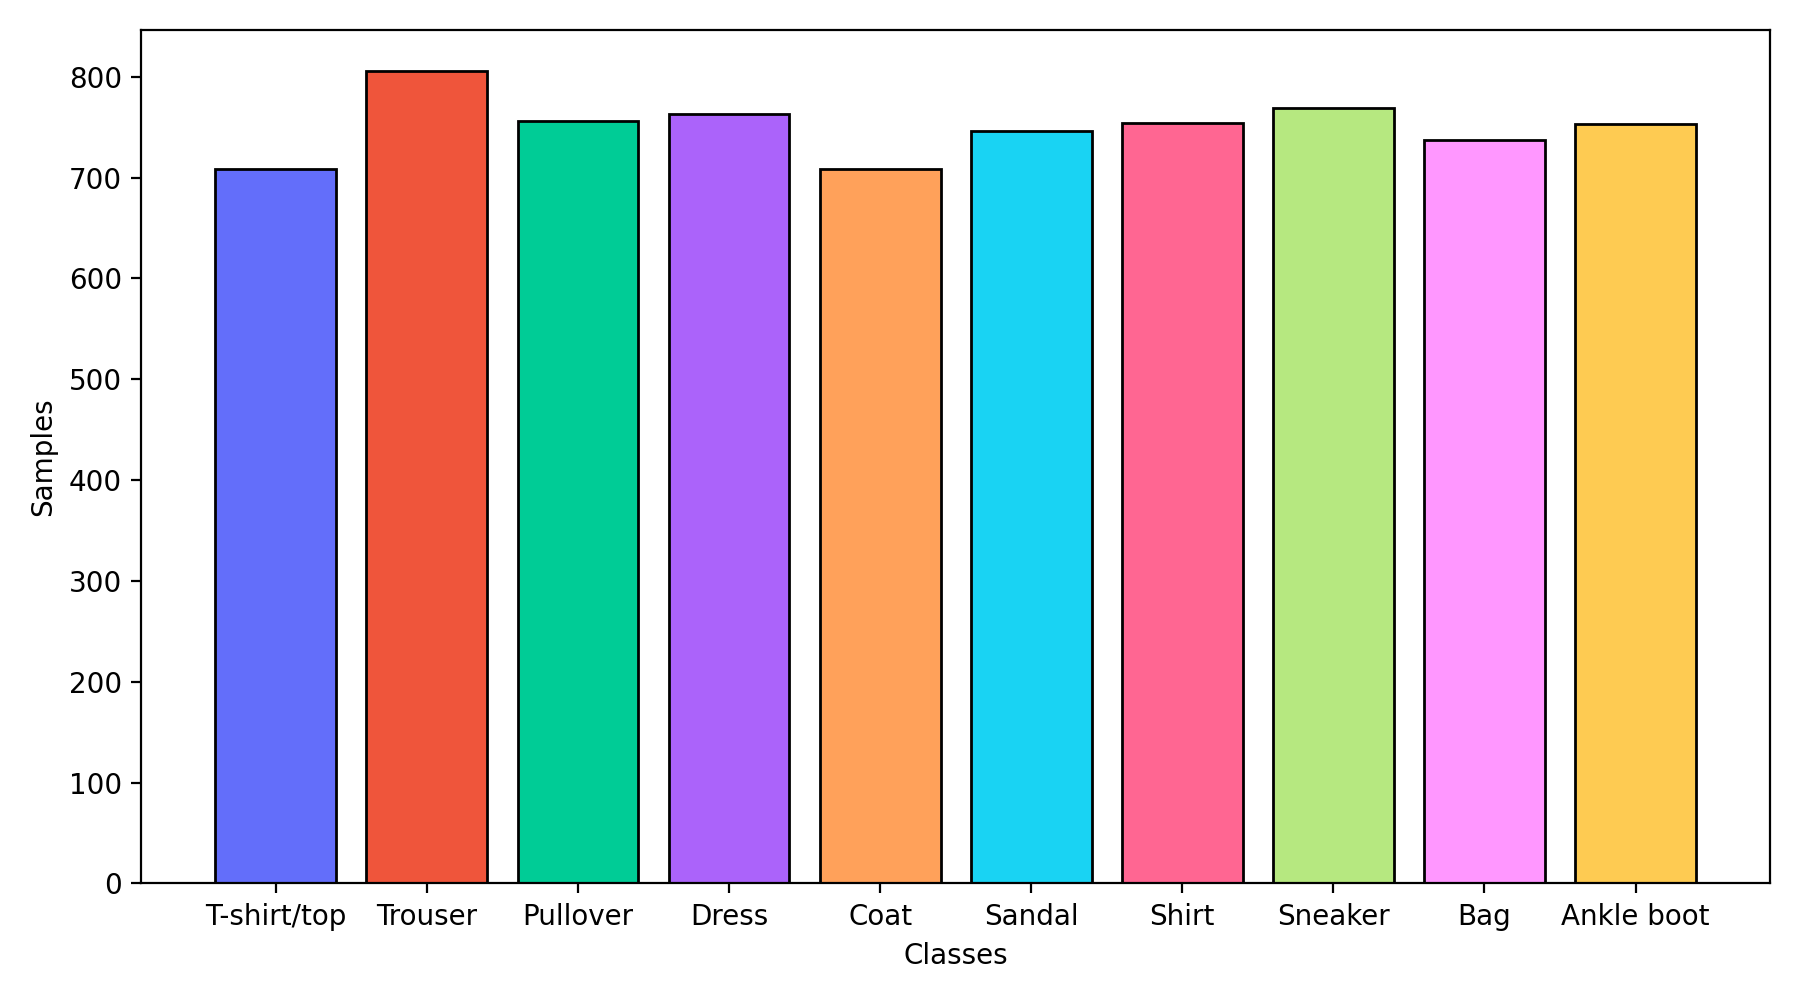
\includegraphics[width=0.65\textwidth]{../plots/reduced_dataset_representativeness.png}
    \caption{\footnotesize Distribution of the reduced training set across the 10 classes.}
    \label{fig:dataset_representativeness}
\end{figure}
\newpage
Once obtained the reduced dataset, I applied some pre-processing transformations. Instead of applying Z-normalization to the data 
on their original scale $(0-255)$, I scaled the pixel values by dividing them by $255$. This scaling step maps the pixel 
values into a more compact range of [0, 1], which is indeed a general good practice for feeding ML models. After scaling, I 
proceeded with centering the data, which is an essential prerequisite for applying PCA. However, I avoided dividing by the standard 
deviation to prevents issues where low standard deviation in pixels (\emph{e.g., corners}) could cause their values to explode.\\[0.2cm]
After completing the data preparation phase, I moved to dimensionality reduction. To explore the impact of different 
configurations I performed a tuning phase, testing various values for \texttt{gamma} (scale parameter for gaussian kernel PCA)
and \texttt{deg} (degree for polynomial kernel PCA). More in details, I tested \texttt{gamma} $\in \{0.001,0.005,0.01,0.05,0.1,0.5,1,5\}$ and
\texttt{deg} $\in \{2,3,4,5\}$. Below I present only the most interesting outcomes from this stage, but for all those 
interested in further details, please refer to the project repository, where all the plots generated during this process are available.

\begin{figure}[!htb]
    \begin{minipage}{0.5\textwidth}
      \centering
      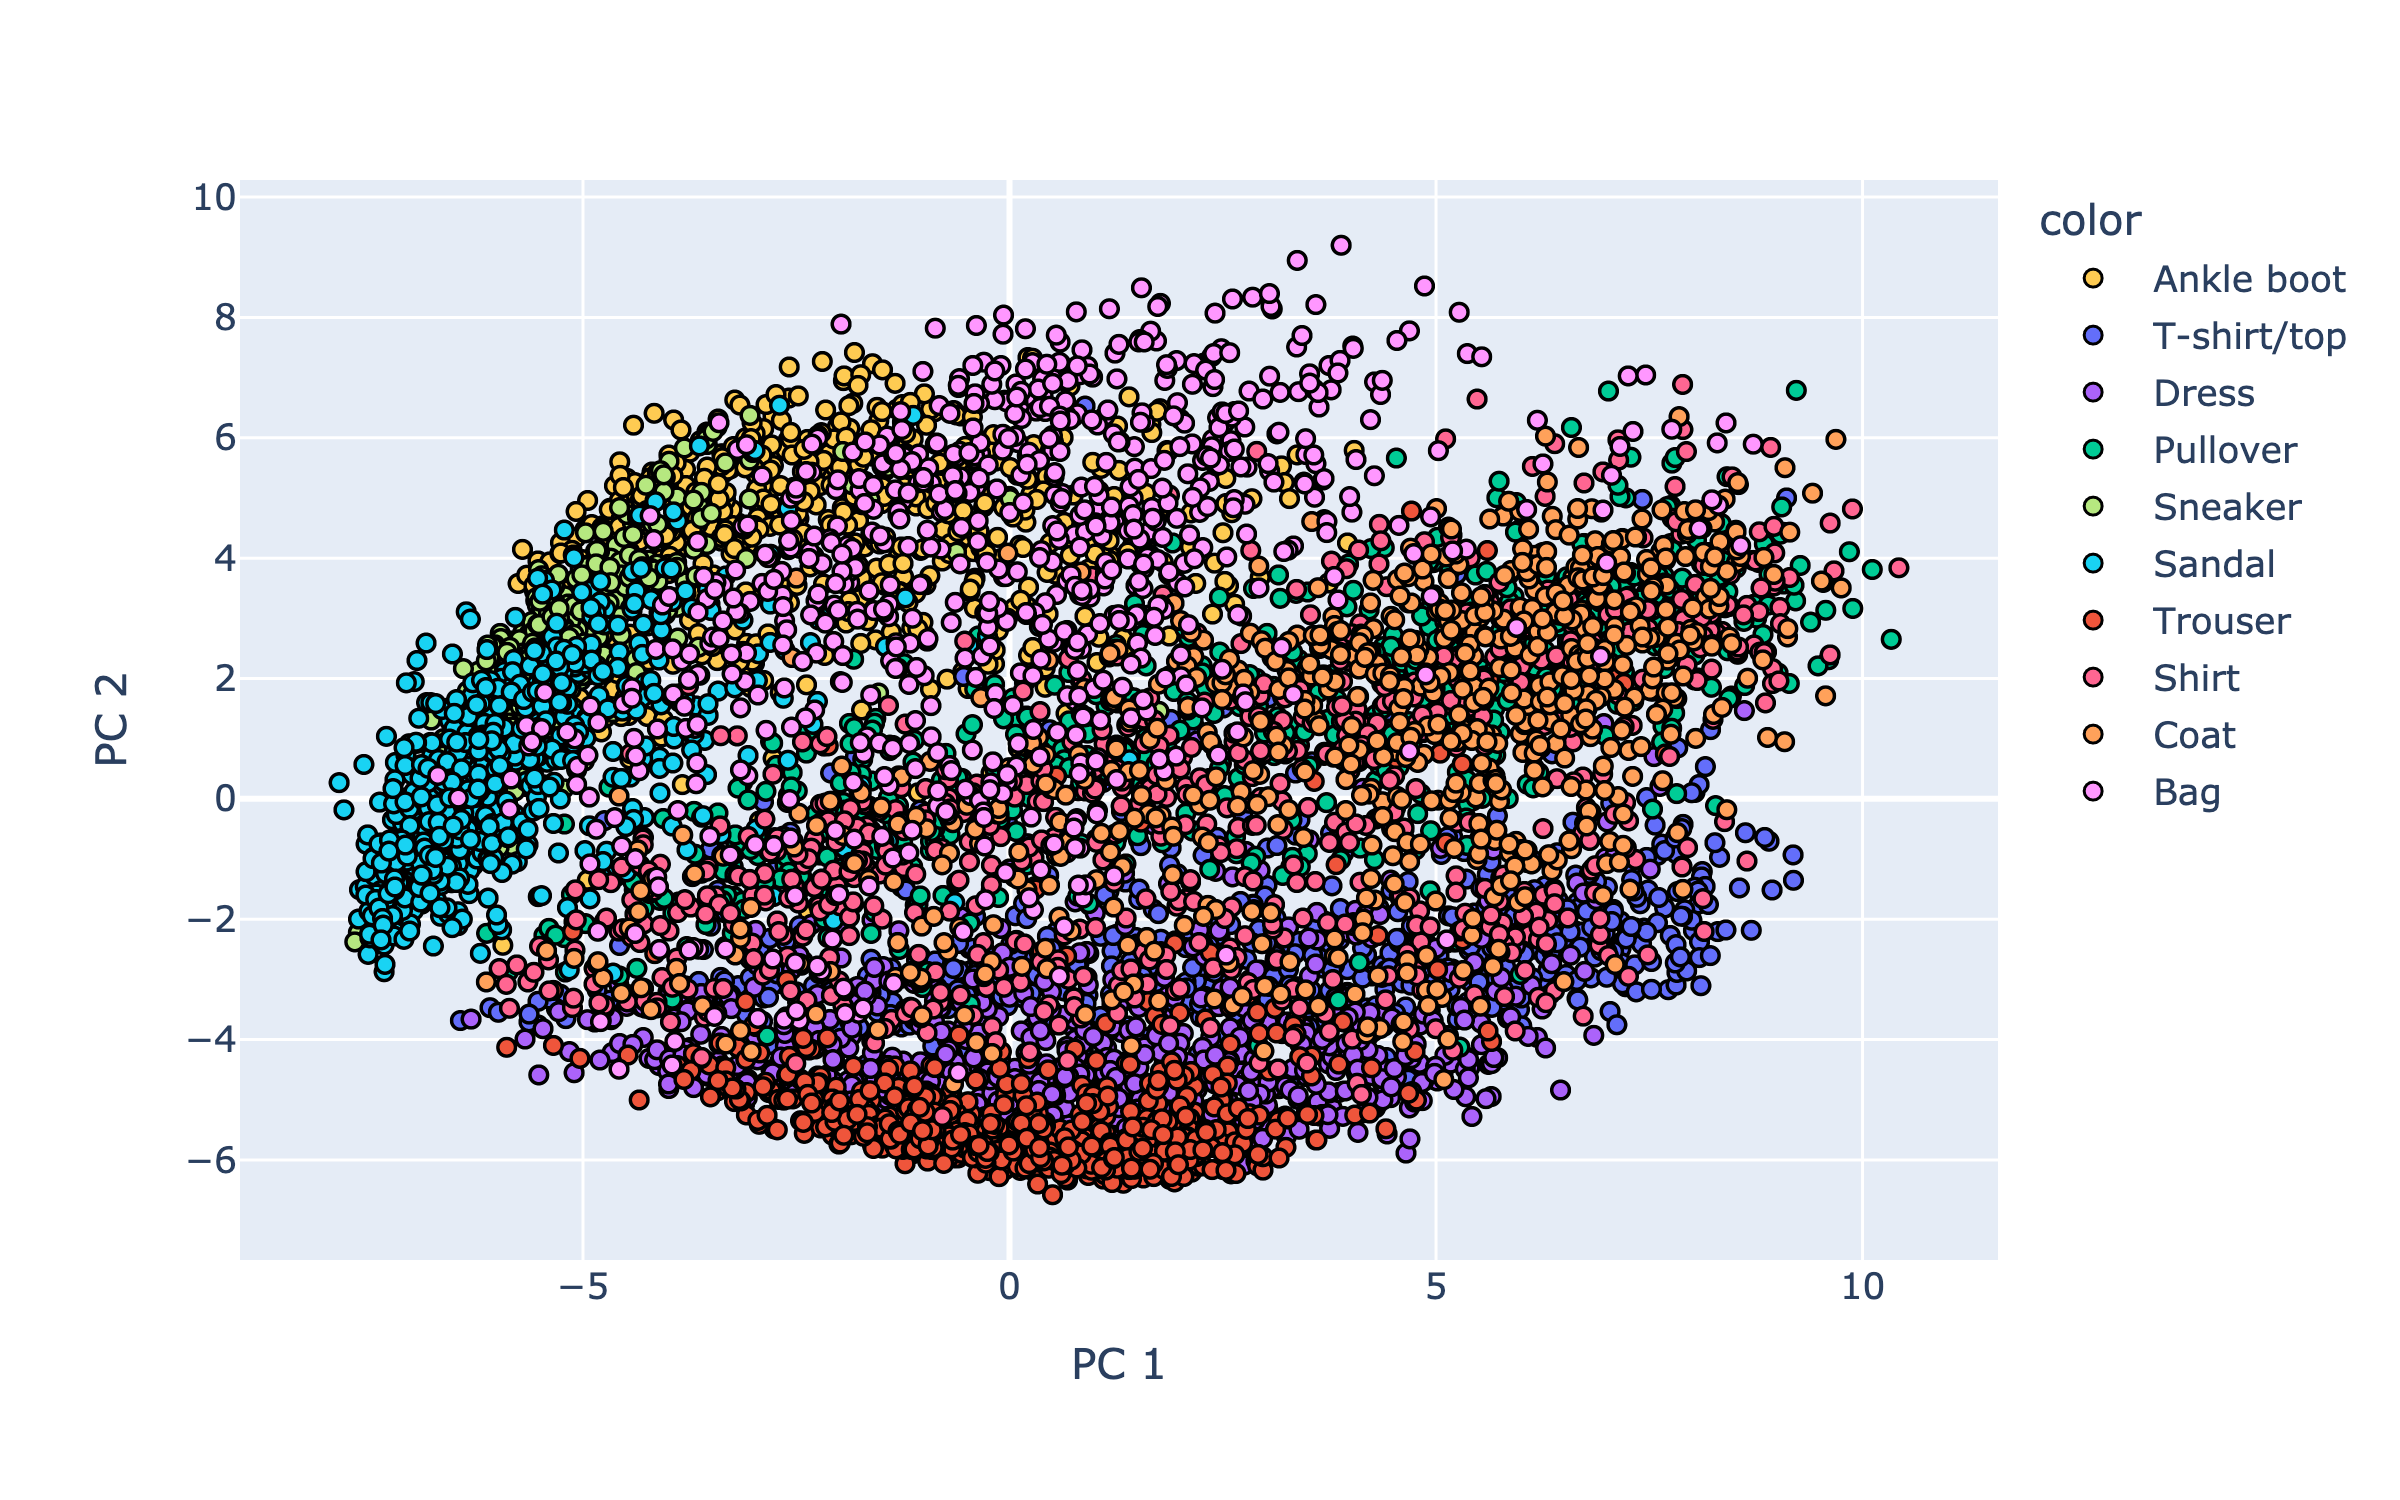
\includegraphics[width=1\linewidth]{images/PCA_2PC.png}
      \caption{\footnotesize Classic PCA, 2d projections }\label{Fig:PCA_2PC}
    \end{minipage}\hfill
    \begin{minipage}{0.5\textwidth}
      \centering
      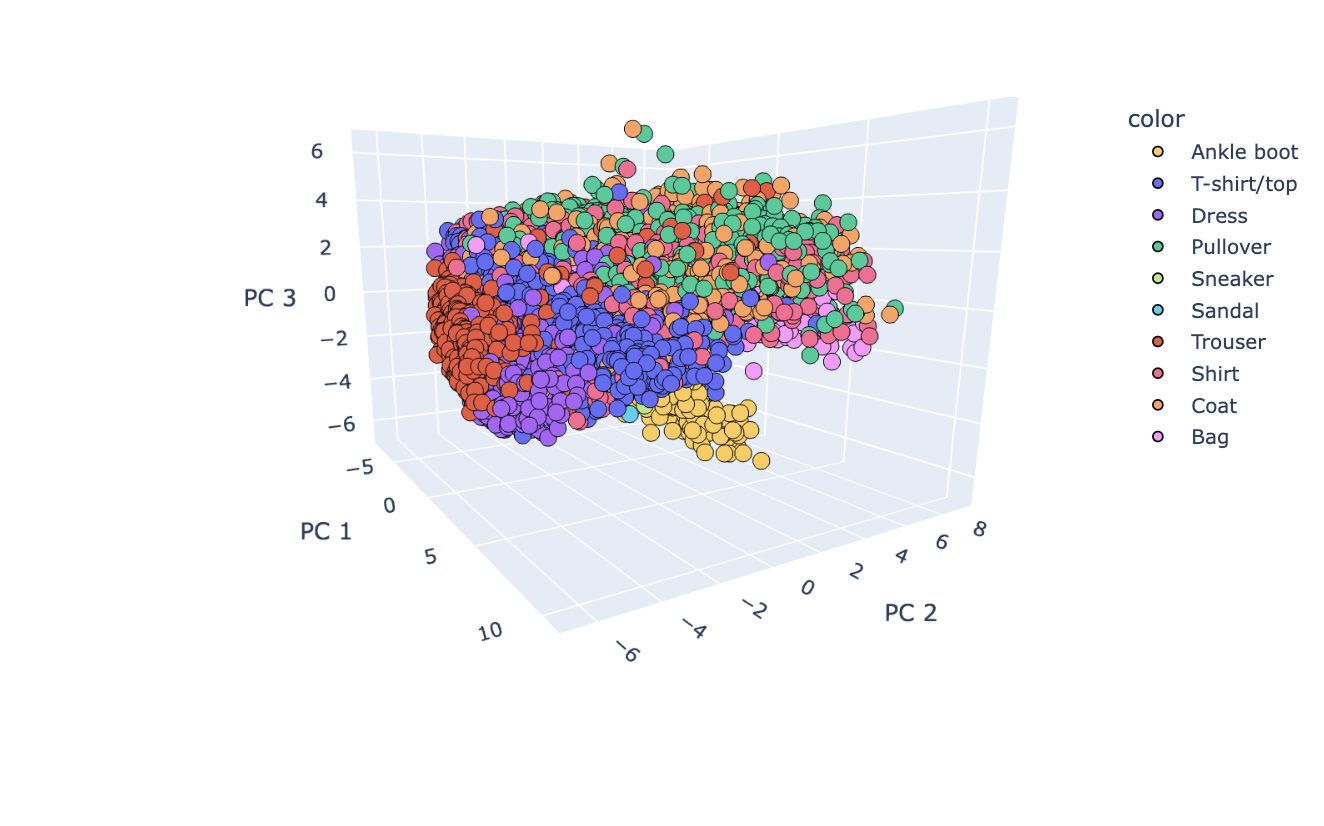
\includegraphics[width=1\linewidth]{images/PCA_3PC.png}
      \caption{\footnotesize Classic PCA, 3d projections}\label{Fig:PCA_3PC}
    \end{minipage}
 \end{figure}

 \begin{figure}[!htb]
    \begin{minipage}{0.5\textwidth}
      \centering
      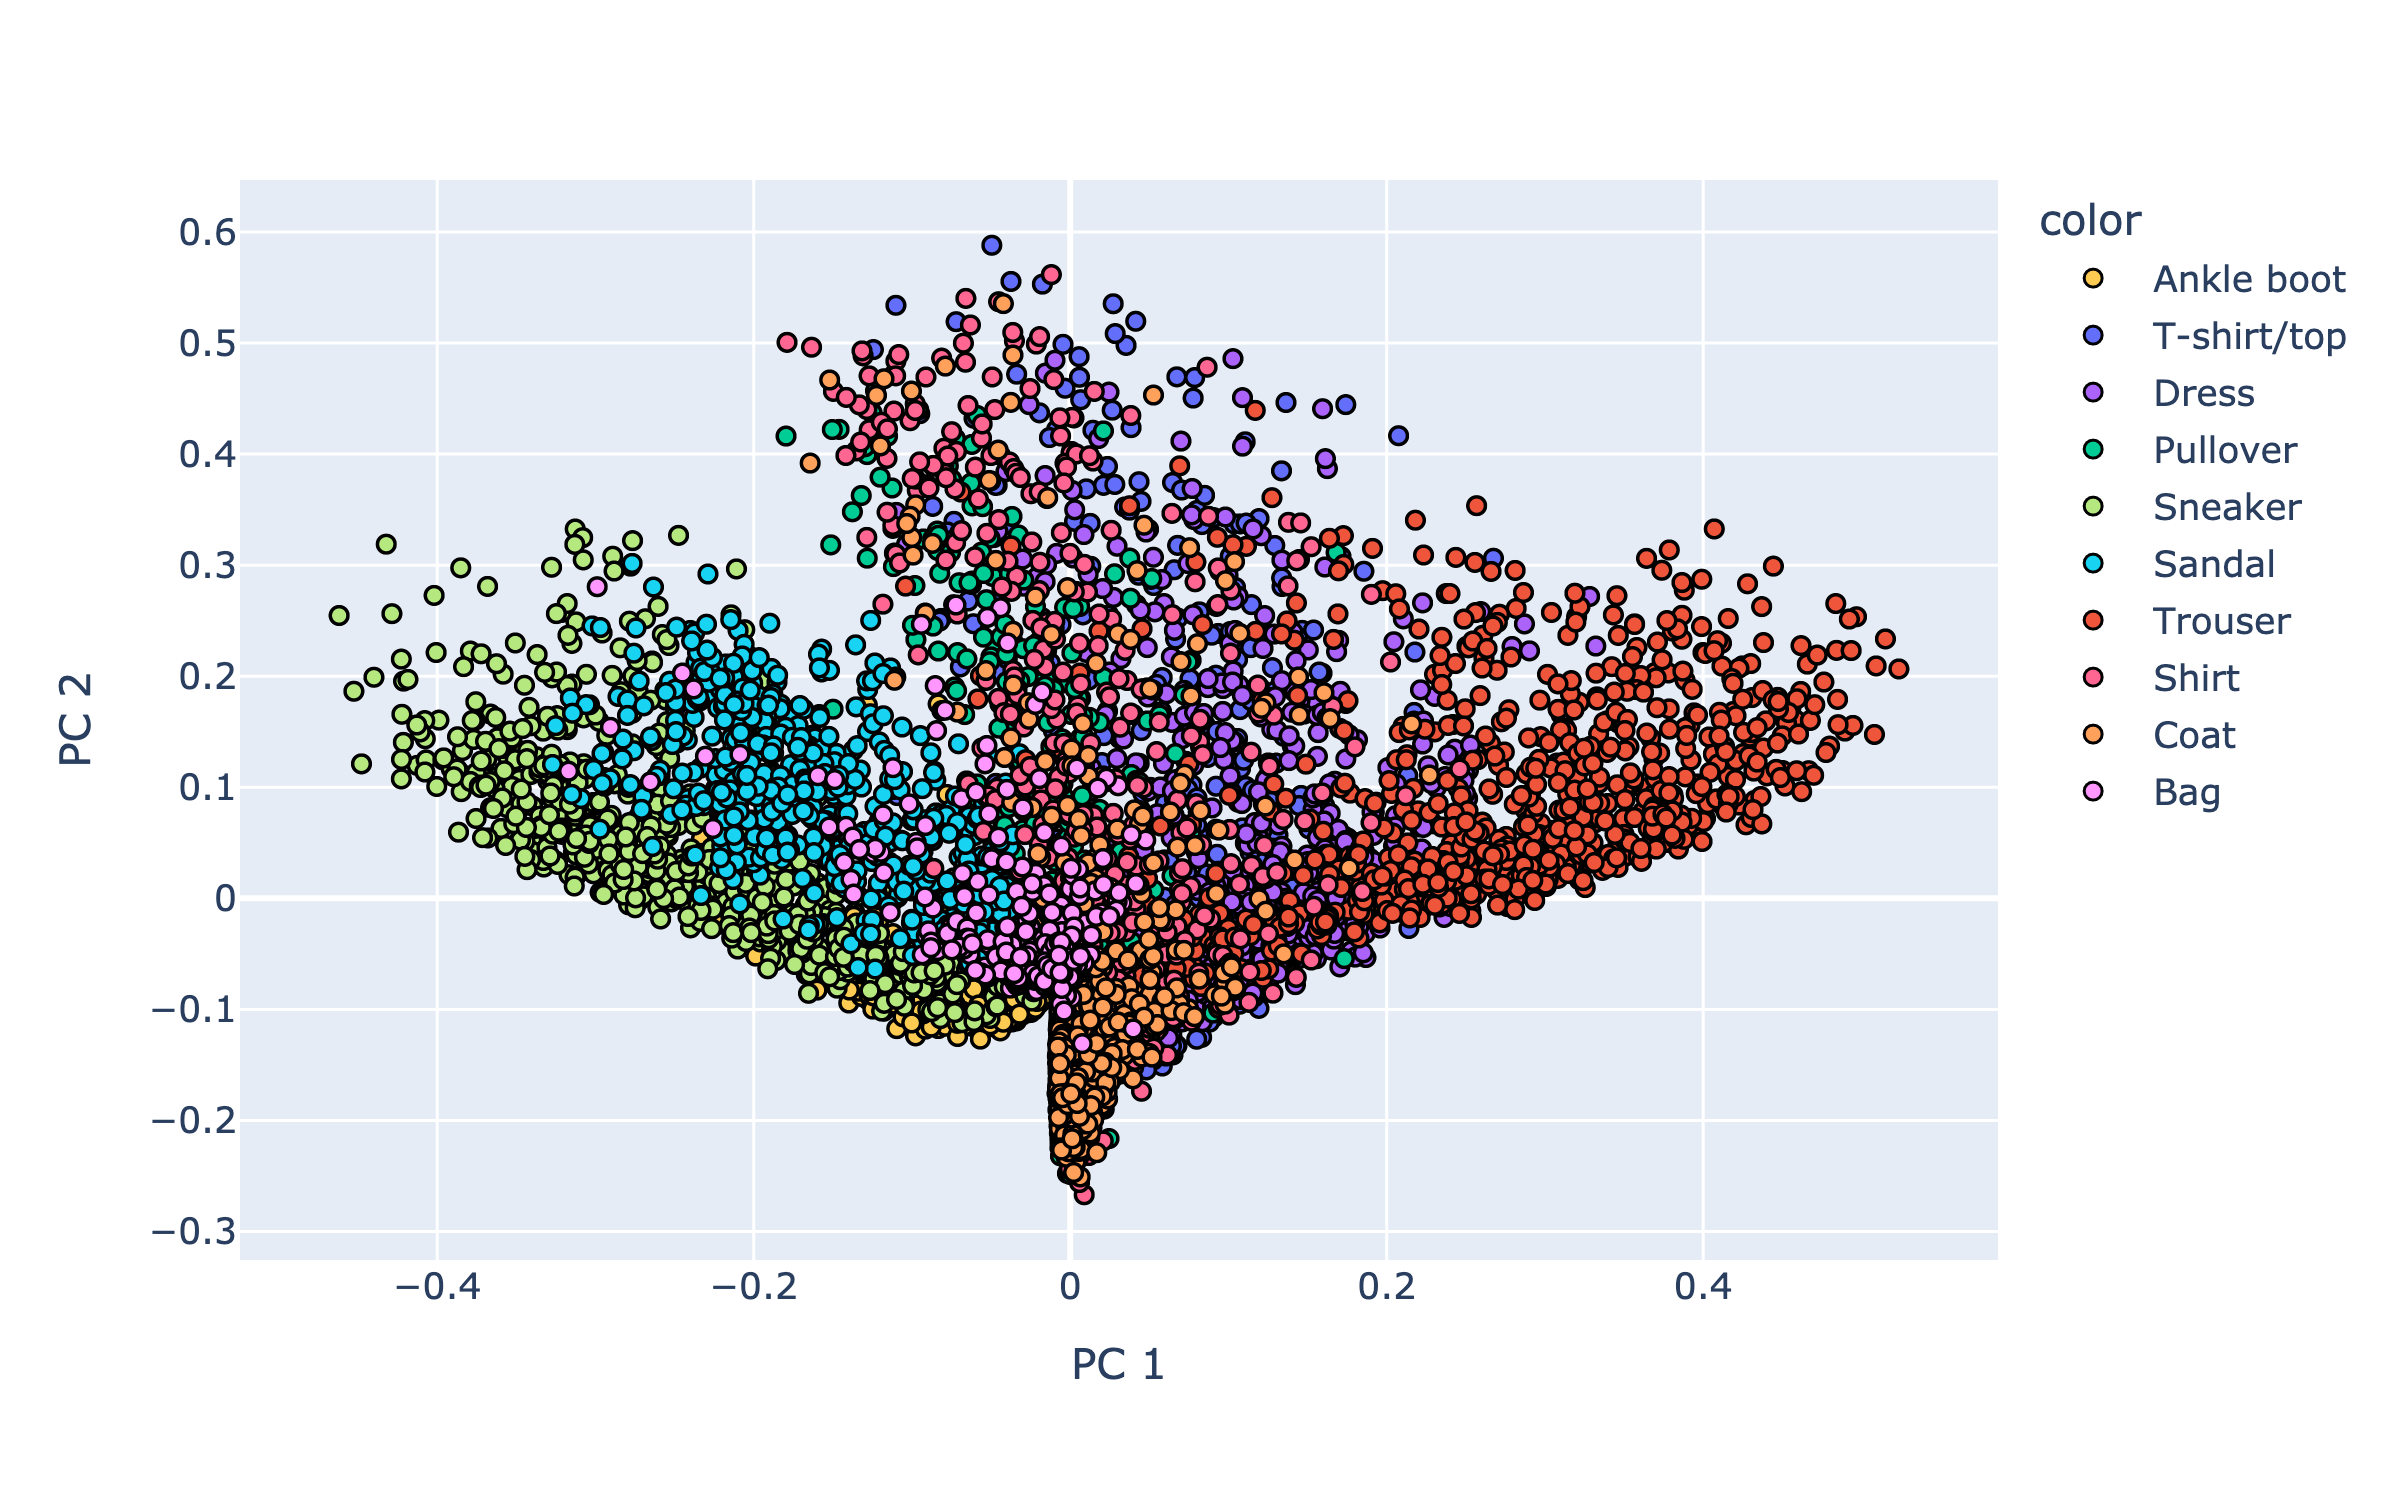
\includegraphics[width=1\linewidth]{images/rbfPCA_2PC.png}
      \caption{\footnotesize rbf kPCA ($\gamma=0.05$), 2d projections}\label{Fig:kPCA_2PC}
    \end{minipage}\hfill
    \begin{minipage}{0.5\textwidth}
      \centering
      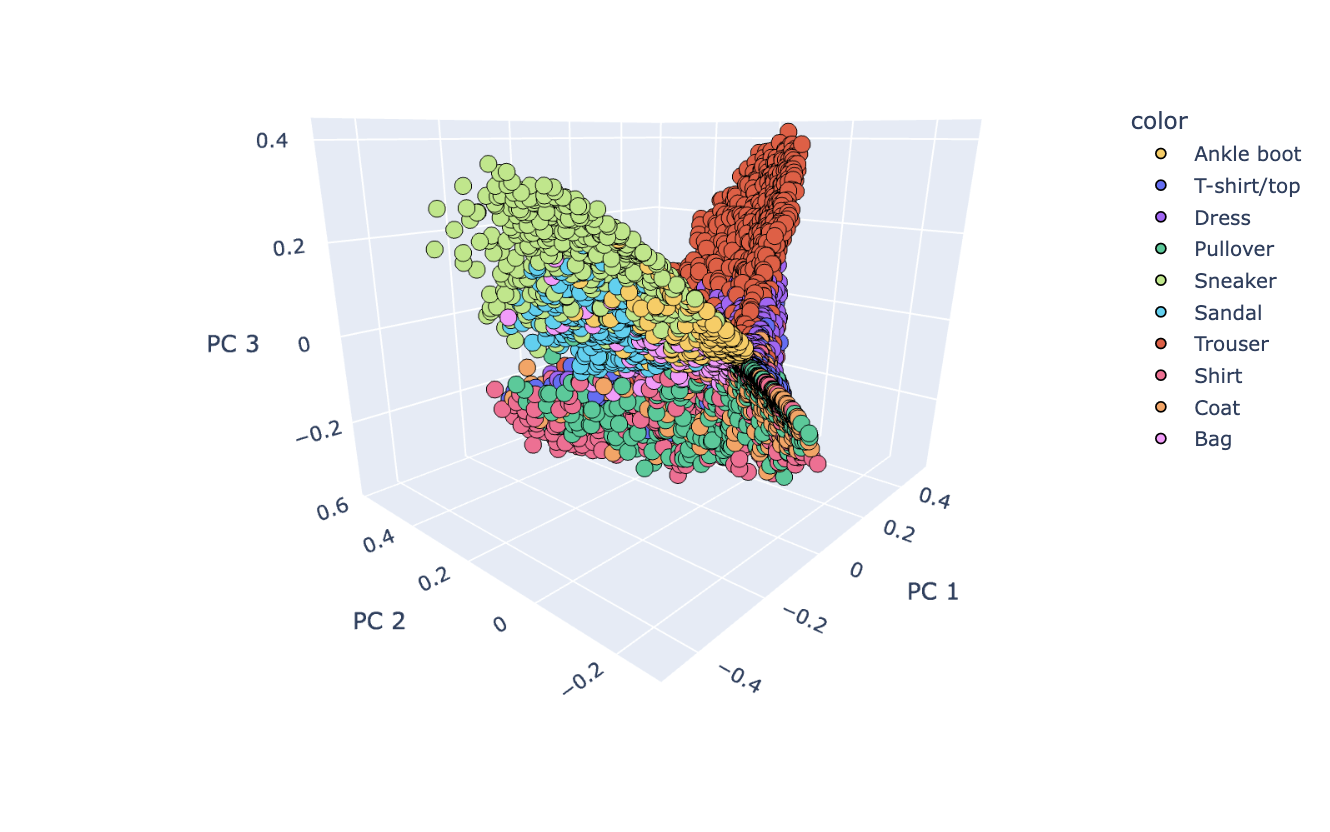
\includegraphics[width=1\linewidth]{images/rbfPCA_3PC.png}
      \caption{\footnotesize rbf kPCA ($\gamma=0.05$), 3d projections}\label{Fig:kPCA_3PC}
    \end{minipage}
 \end{figure}

Despite its simplicity, PCA managed to highlight some distinct groupings, as shown in \Cref{Fig:PCA_2PC,Fig:PCA_3PC}. Clear 
clusters are visible for categories such as bags, trousers, sandals, and ankle boots, with points in these groups appearing tightly concentrated. 
However, significant overlap remains among other classes, suggesting that PCA alone may not fully distinguish between all categories. I also 
experimented with polynomial PCA: a degree of 2 produced results similar to classical PCA, offering no notable improvement 
in cluster separation. Increasing the polynomial degree did not yield any substantial enhancement, either. Gaussian PCA, on the other hand, 
provided refined separation, especially for bags, trousers, sandals, and ankle boots, whose clusters appear even more distinctly defined. 
The dress category also shows improved separation, albeit less clearly in the plots. \Cref{Fig:kPCA_2PC,Fig:kPCA_3PC} reveal an 
interesting pattern: ankle boots, sandals, and sneakers form a cohesive region, while trousers are positioned more independently. This makes sense, 
given that ankle boots, sandals, and sneakers are all types of footwear, while trousers have features that set them apart from all the other labels 
in the dataset (if \emph{Fashion-MNIST} had included shorts or underwear, there might have been an overlapping with trousers).
Upper-body items like shirts, t-shirts, coats, and pullovers continue to overlap significantly, which is reasonable as they share 
similar shapes and visual traits.
%\newpage
    \section{Bridging unsupervised and supervised}\label{clustering}
After performing dimensionality reduction using kernel PCA and retaining the first 10 principal components, I proceeded to assign labels 
to the resulting data points. Rather than using the true labels, the objective was to cluster the data into 10 groups and then evaluate how well these clusters captured the 
data's underlying structure. To achieve this, I selected agglomerative clustering over the usual K-means for several reasons:
\begin{enumerate}
    \item while K-means performs well with spherical clusters, the transformed data from kernel PCA typically exhibits complex, non-spherical geometries. 
    Agglomerative clustering is better suited to these shapes, as it captures more effectively irregular and overlapping clusters, leading to a closer 
    approximation of the true data structure;
    \item  agglomerative clustering is robust to outliers, making it particularly suitable for a high-dimensional and potentially noisy dataset like ours. 
    Unlike K-means, where outliers influence centroids and lead to distorted assignments, agglomerative clustering is less sensitive to such anomalies, maintaining more reliable clustering results;
    \item agglomerative clustering offered flexibility in the choice of the distance metric. Nevertheless, I still opted to use Euclidean distance specifically to 
    leverage Ward’s linkage, which minimizes the total within-cluster variance (a desirable property in this analysis). Ward’s linkage also tends to produce balanced clusters, 
    aligning with my aim to create clusters that mirror the true, balanced structure of the dataset.
\end{enumerate}

\Cref{fig:sankey_diagram} shows a Sankey diagram representing the flow between the true labels and the cluster assignments, 
making it easier to inspect if there is any relevant correspondence. \Cref{fig:cluster_composition}, instead, shows the composition of each cluster with respect to the true labels, providing an additional, intuitive way to evaluate 
the quality of the clustering procedure.
\begin{figure}[ht]
    \centering
    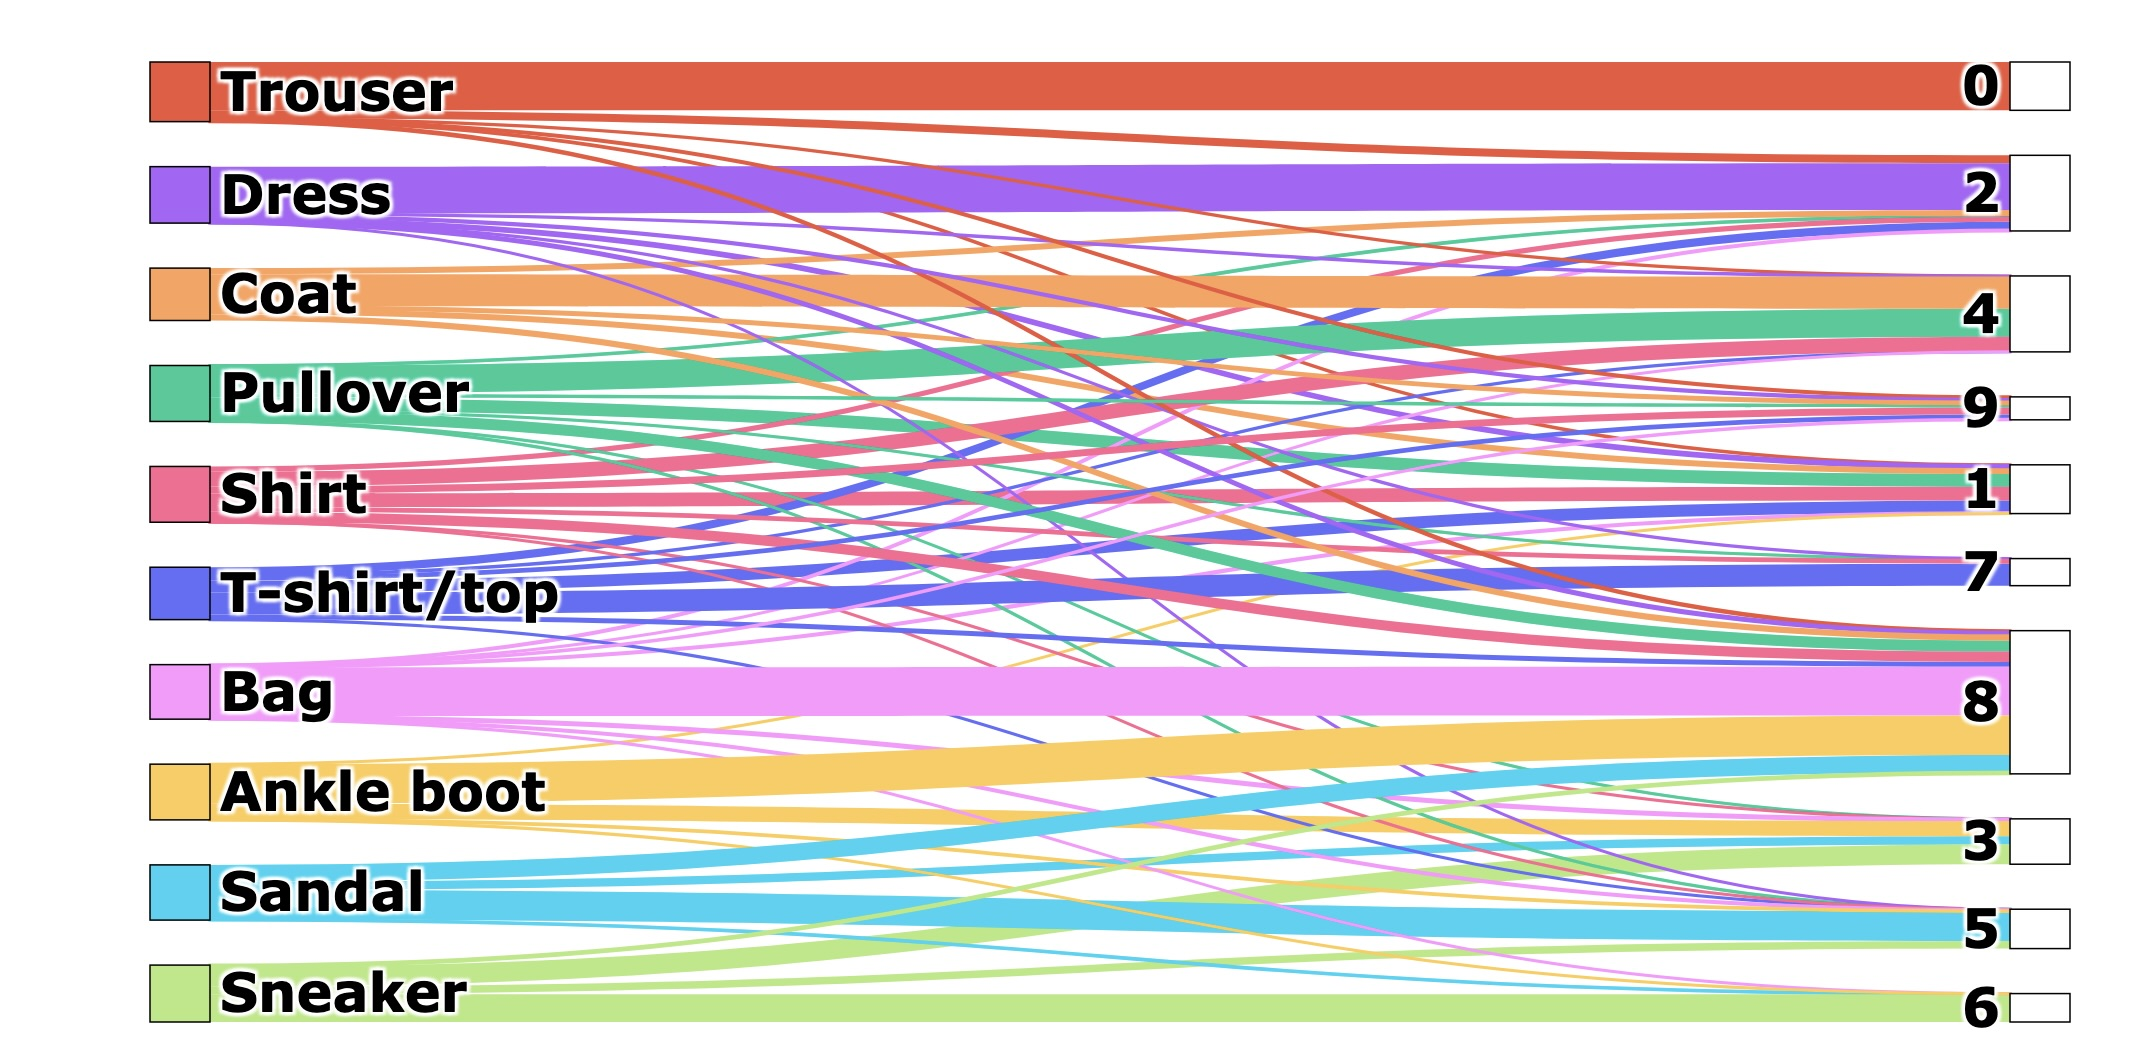
\includegraphics[width=0.62\textwidth]{images/sankey_diagram.png}
    \caption{\footnotesize Sankey diagram}
    \label{fig:sankey_diagram}
\end{figure}

\begin{figure}[ht]
    \centering
    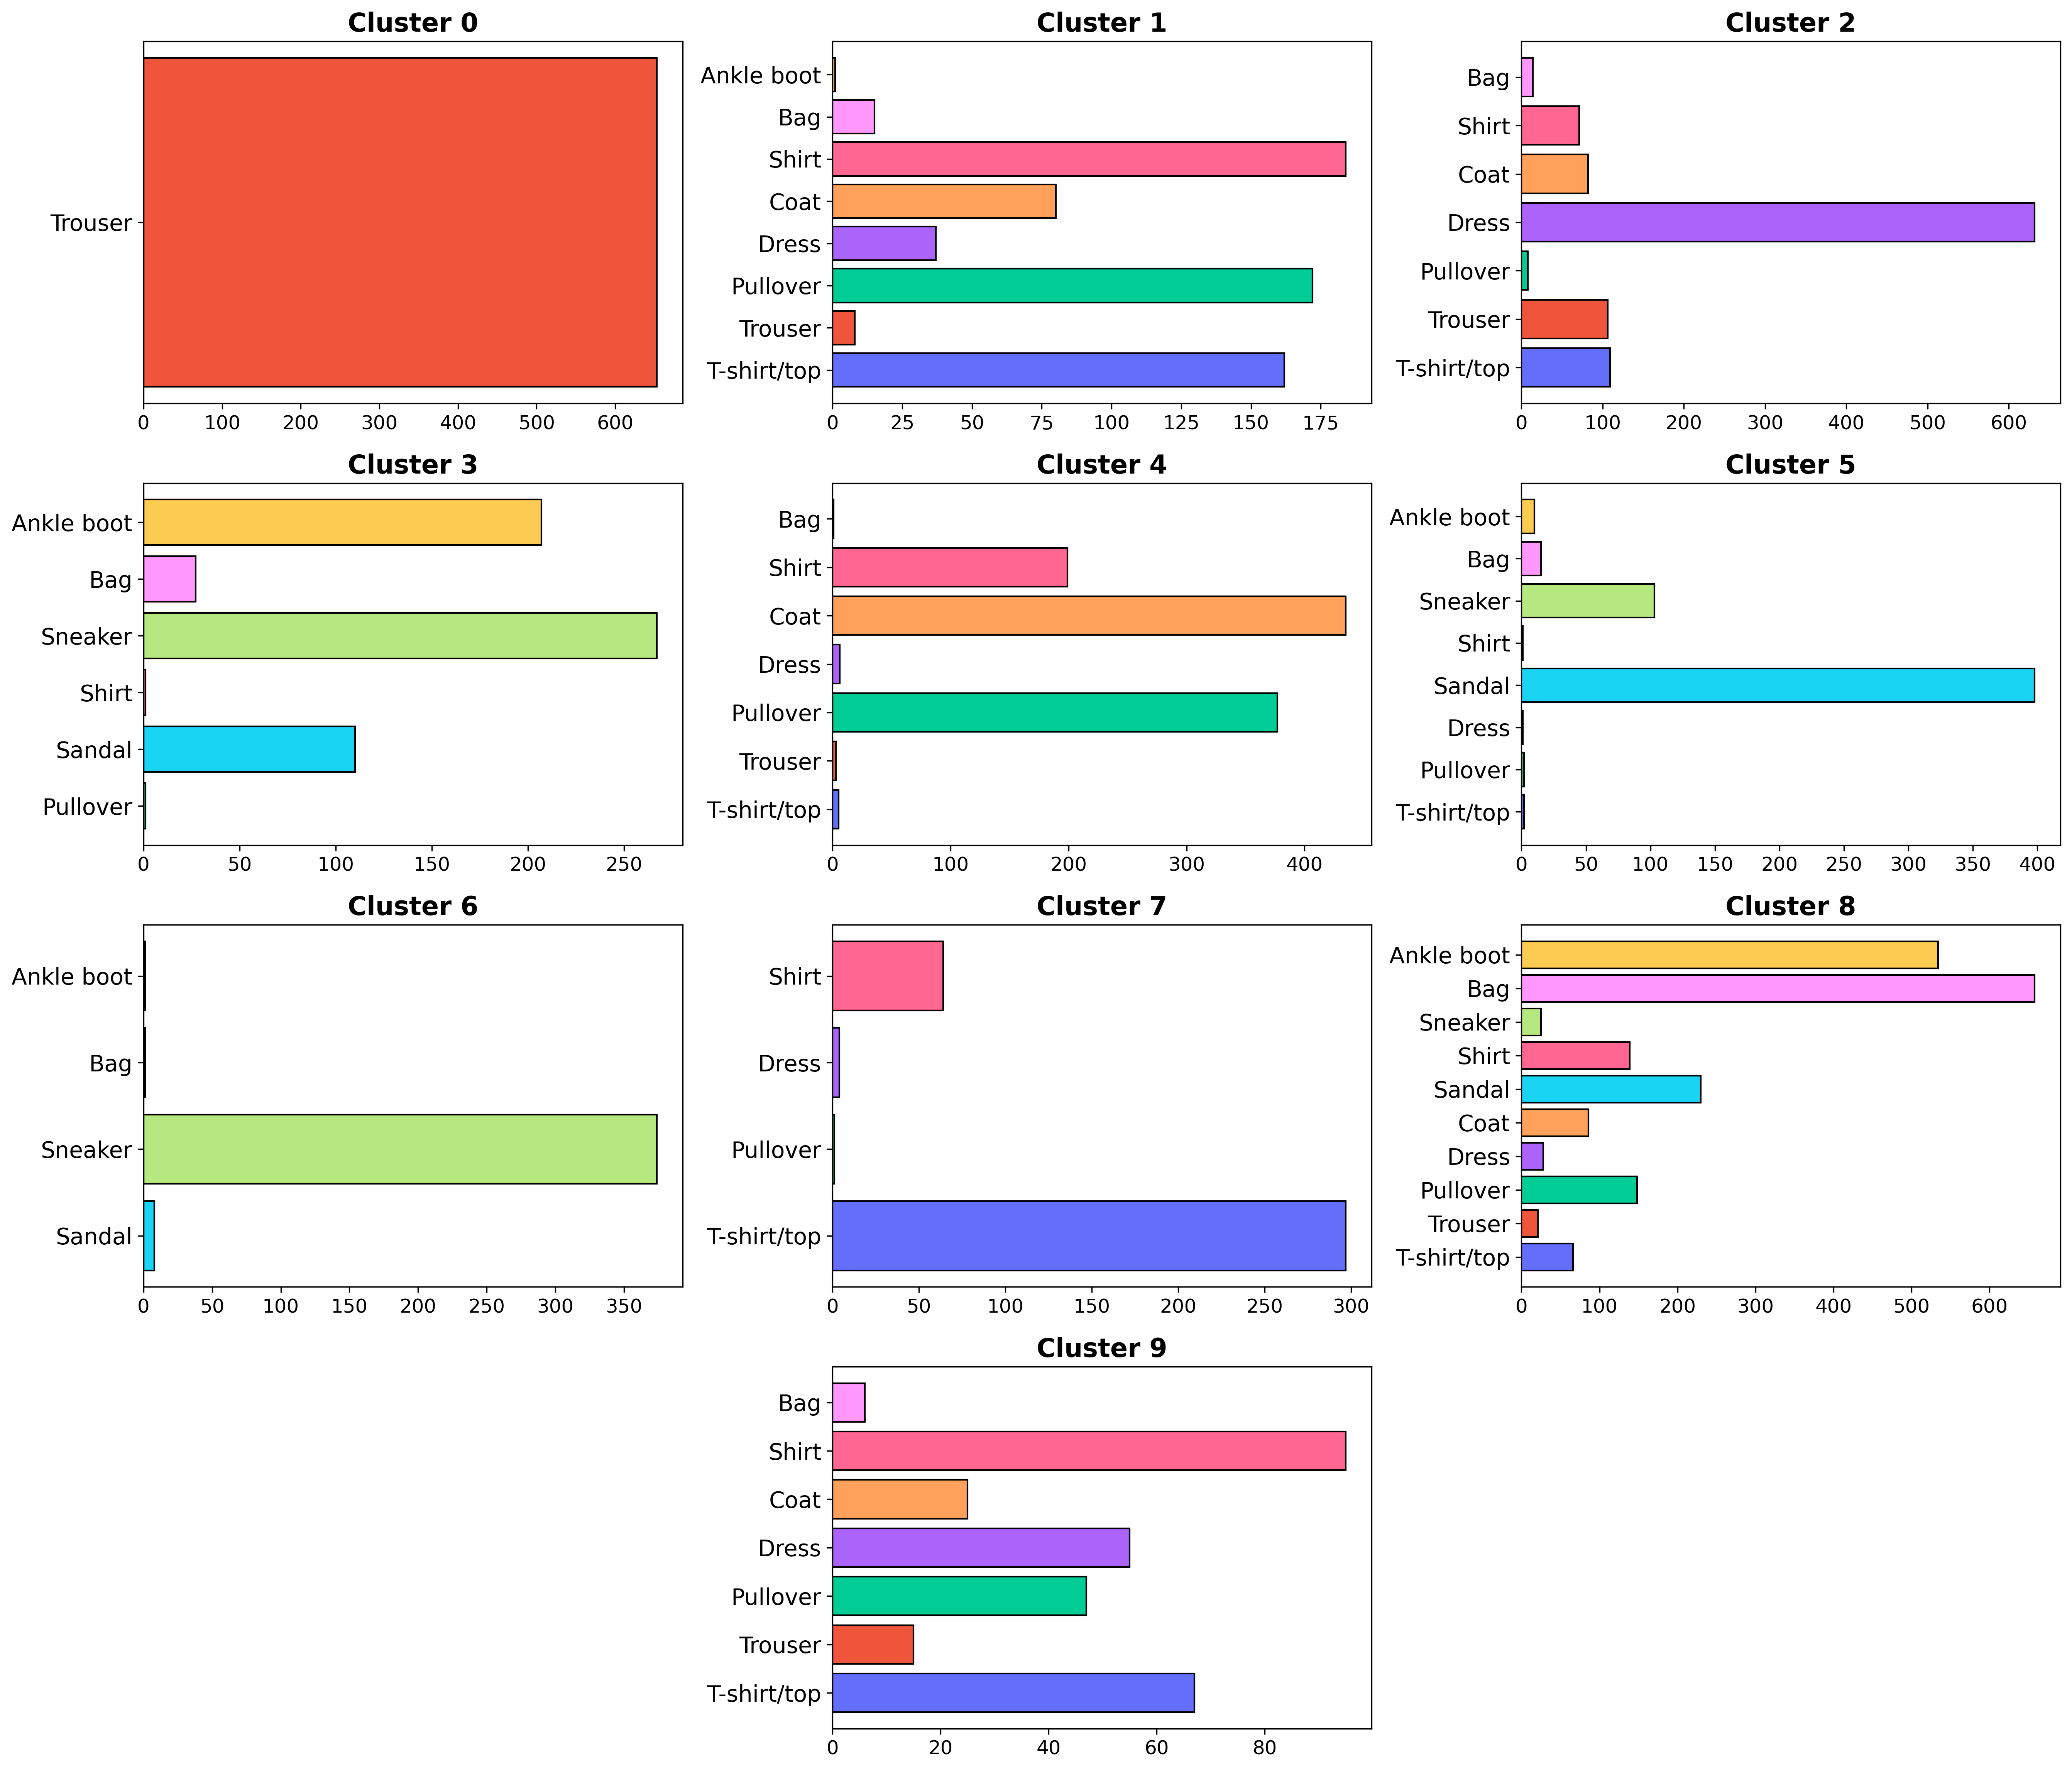
\includegraphics[width=0.85\textwidth]{images/clusters_composition_AC_3x4grid.png}
    \caption{\footnotesize Cluster composition w.r.t. the true labels}
    \label{fig:cluster_composition}
\end{figure}

The cluster composition largely reflects the data geometry discussed in \Cref{data_geometry}. Cluster 0 consists solely of trousers, confirming them as the most 
separable category. Clusters 3, 5, and 6 are instead dominated by footwear, with sneakers being the majority class for clusters 3 and 6 (a redundancy better
discussed in later sections). Clusters 1, 4, and 9 exhibit a balanced mix of shirts, coats, pullovers and T-shirts/tops, underscoring 
the difficulty in distinguishing upper-body clothing items. Cluster 8 shows an interesting deviation: while 
bags appeared well-separated in 2D and 3D projections, it contains a notable proportion of ankle boot samples.
This overlap may be due to actual shared visual features between bags and boots. However, with just 10 components, we may be missing finer details 
that that could improve class separation. This is supported by the spectrum in \Cref{fig:kpa_spectrum}, where the optimal `elbow' 
for component selection likely exceeds 10 components, indicating the need of additional components to improve clustering fidelity.

\begin{figure}[ht]
    \centering
    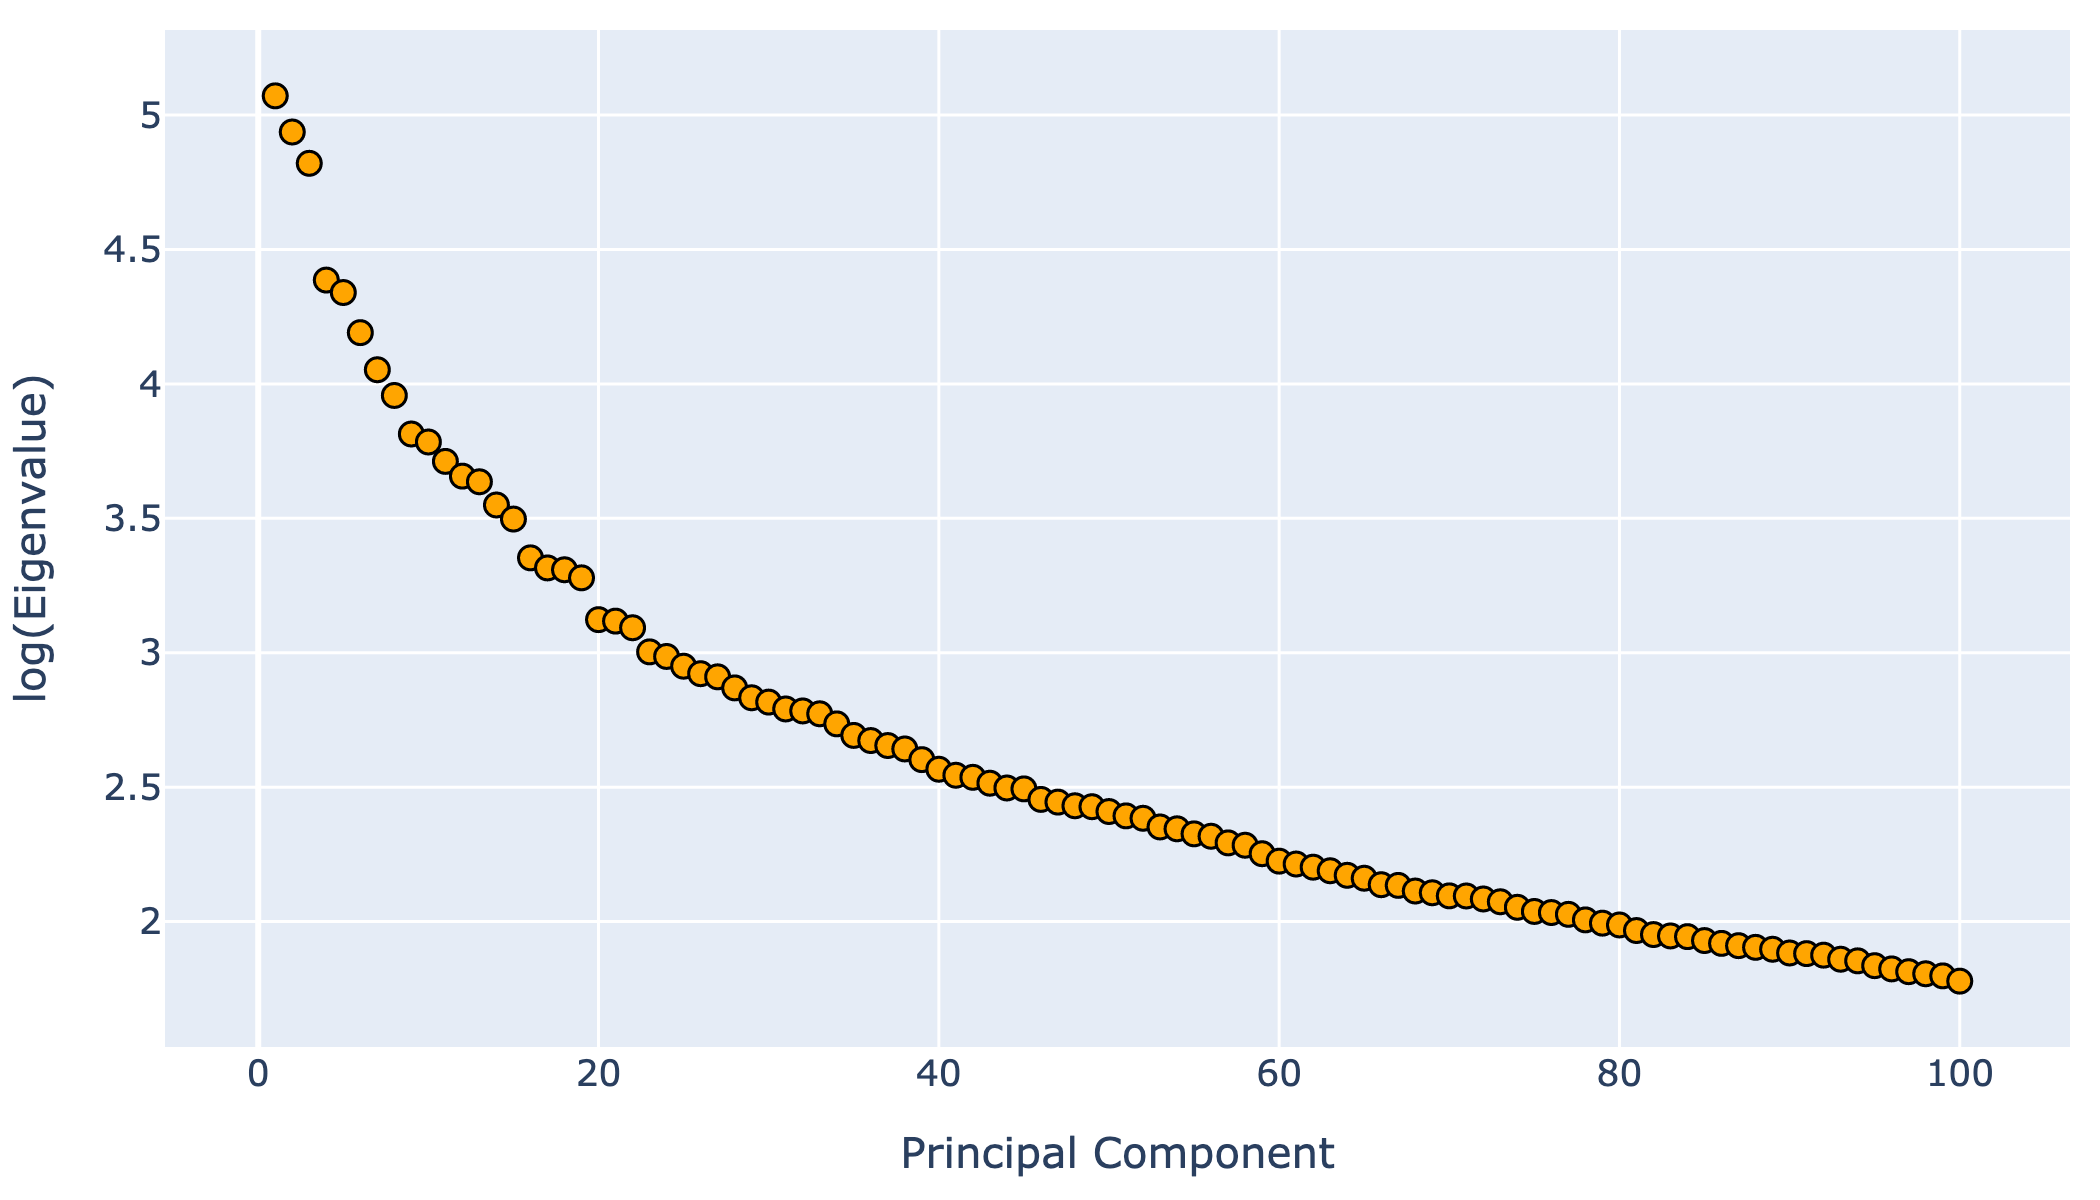
\includegraphics[width=0.5\textwidth]{images/best_kPCA_spectrum.png}
    \caption{\footnotesize Spectrum of the log(eigenvalues) from kernel PCA}
    \label{fig:kpa_spectrum}
\end{figure}
\newpage
To further investigate this, I performed an analysis of the intrinsic dimensionality of the data using the two-NN algorithm 
provided by the \texttt{DADApy} package. The results indicated an intrinsic dimensionality of approximately 15, reinforcing the 
hypothesis that additional components could capture meaningful variation in the data and improve clustering performance. I finally computed 
some quantitative metrics to assess the clustering performance, which are summarized in \Cref{tab:clustering_metrics}.
\begin{table}[h!]
    \centering
    \begin{tabular}{|l|c|}
    \hline
    \textbf{Metric}                  & \textbf{Score}         \\ \hline
    Normalized Mutual Information    & 0.5029                 \\ 
    Adjusted Rand Score              & 0.3257                 \\
    Homogeneity                      & 0.4855                 \\
    Completeness                     & 0.5215                 \\
    V-Measure                        & 0.5029                 \\ \hline
    \end{tabular}
    \caption{Clustering Evaluation Metrics}
    \label{tab:clustering_metrics}
\end{table}

    \section{(Supervised) classification}\label{hybrid_model_tuning}
I implemented and compared three different supervised classification models: \emph{Support Vector Classification (SVC)},
\emph{Fully Connected Neural Networks (FCNN)} and \emph{Convolutional Neural Network (CNN)}. These models were trained using as target labels the 
cluster-assigned labels from the unsupervised learning phase, rather than the original labels. The input to the models, 
instead, consisted of the original images, not the 10-dimensional projections actually used for the clustering phase. The objective was to tune different 
configurations for each model and compare their performance in terms of \emph{balanced accuracy} and computational cost. Instead of a static
train-test split for the tuning, I considered to perform \emph{5-fold cross validation} to ensure robustness and generalization of the results.

\subsection{Support Vector Classification (SVC)}\label{hybrid_model:svc}
Parameter search was performed using the \texttt{GridSearchCV} function from \texttt{scikit-learn}. The grid of hyperparameters was designed 
to evaluate two kernels, Polynomial and Gaussian, with the following configurations:
\begin{itemize}
    \item \textbf{Polynomial kernel}
    \begin{itemize}
        \item Regularization parameter \texttt{C} $\in \{0.1, 1, 10, 50\}$
        \item Polynomial degree \texttt{deg} $\in \{2, 3, 4\}$
    \end{itemize}
    \item \textbf{Gaussian kernel}
    \begin{itemize}
        \item Regularization parameter \texttt{C} $\in \{0.1, 1, 10, 50\}$
        \item Scale parameter \texttt{gamma} $\in \{0.005,0.01,0.05,0.1,0.5,1,5\}$
    \end{itemize}
\end{itemize}

The values for \texttt{gamma} were selected basing on the same range used during dimensionality reduction with the gaussian kernel PCA. 
This alignment seemed reasonable to maintain the structural relationships of the data between the two steps, making it more likely that 
the \emph{SVC} would effectively classify the data based on the transformed feature space. The grid for the regularization parameter \texttt{C} 
was designed to explore a wide range of scales, from smaller values encouraging a simpler decision boundary, to larger values accommodating 
more complex boundaries. The best configuration found during the tuning phase was a gaussian kernel with \texttt{gamma}=0.05 and 
\texttt{C}=10, which yielded the best performance.
\newpage

\subsection{Fully Connected Neural Network (FCNN)}\label{hybrid_model:fcnn}
For the \emph{FCNN}, rather than building two networks with different configurations (as suggested), I wanted to perform a deeper analysis 
through a more extensive hyperparameter tuning process. Although the model was implemented in \texttt{PyTorch}, I managed to use \texttt{GridSearchCV}
by leveraging the \texttt{skorch} library, which provides a wrapper around \texttt{PyTorch} and offers a \texttt{sklearn}-compatible 
interface. I designed the network with a single hidden layer and explored various configurations, tuning both some parts of the architecture 
(hidden layer size, type of non-linearity and dropout rate) and some training hyperparameters including batch size and learning rate. 
The hyperparameter grid I used for tuning was the following:
\begin{itemize}
    \item \textbf{Hidden dimension}: $\{128, 256, 512\}$
    \item \textbf{Non linearity}: \{\texttt{ReLU()}, \texttt{Sigmoid()}, \texttt{Tanh()}\}
    \item \textbf{Dropout}: $\{0.0, 0.5\}$
    \item \textbf{Learning Rate}: $\{0.001,0.01\}$
    \item \textbf{Batch Size}: $\{64, 128, 256\}$
\end{itemize}

Among all the networks tested in the cross-validation, the best performance was achieved by the network with 128 hidden units, Sigmoid 
activation function and dropout rate of 0.5, trained with a learning rate of 0.01 and a batch size of 64.

\subsection{Convolutional Neural Network (CNN)}\label{hybrid_model:cnn}

For the \emph{CNN} architecture, I designed a network consisting of two convolutional layers followed by a two connected layers. Given the 
reduced image size of 28x28 pixels, I chose a standard solution that preserves the spatial dimensions of the image as much as possible during 
the convolutional steps. To achieve this, I relied on a kernel size of 3, a stride of 1 and padding of 1 for the convolutional layers. 
After each convolutional layer, a pooling layer is applied in order to reduce the spatial dimensions. Specifically, I used pooling layers 
with a kernel size of 2 and a stride of 2, which halves the width and height of the feature maps. For the convolutional layers, I started 
with 16 output channels in the first layer and doubled the number of channels to 32 in the second layer. Then the fully connected layers take 
the flattened output from the last convolutional layer and map it to the number of output classes through 128 hidden neurons. For hyperparameter 
tuning, I conducted a grid search focusing on the activation function, the type of pooling and the presence or not of batch normalization, 
as well as training hyperparameters such as learning rate and batch size. In summary, the grid I used for hyperparameter tuning was:

\begin{itemize} 
    \item \textbf{Non-linearity}: $\{\texttt{ReLU()}, \texttt{Sigmoid()}, \texttt{Tanh()}\}$ 
    \item \textbf{Pooling}: $\{\texttt{MaxPool2d()}, \texttt{AvgPool2d()}\}$ 
    \item \textbf{Batch Normalization}: $\{\texttt{True}, \texttt{False}\}$ 
    \item \textbf{Learning Rate}: $\{0.001, 0.01\}$ 
    \item \textbf{Batch Size}: $\{64, 128, 256\}$ 
\end{itemize}

After performing cross-validation, the configuration achieving the best performance resulted to be the network with 
\texttt{ReLU()} activation function, \texttt{AvgPool2d()} pooling and batch normalization, trained with and a learning rate 
of 0.01 and a batch size of 64.
\newpage
The performance of the three models is outlined in \Cref{tab:model_comparison}.
\begin{table}[h!]
    \centering
    \begin{tabular}{|c|c|c|c|}
    \hline
    \textbf{Model} & \textbf{Balanced Accuracy} & \textbf{Training Time (s)} & \textbf{Inference Time (s)}  \\
    \hline
    SVC & 0.9415 $\pm$ 0.0034 & 3.8215 $\pm$ 0.0210 & 1.2606 $\pm$ 0.0067 \\
    FCNN & 0.8970 $\pm$ 0.0068 & 2.2041 $\pm$ 0.0246 & 0.0094 $\pm$ 0.0002 \\
    CNN & 0.9033 $\pm$ 0.0072 & 4.2941 $\pm$ 0.0254 & 0.0358 $\pm$ 0.0018 \\
    \hline
    \end{tabular}
    \caption{\footnotesize Comparison of SVC, FCNN, and CNN in terms of balanced accuracy, training time, and inference time. 
    All the values are expressed as confidence intervals at 95\% level.}
    \label{tab:model_comparison}
\end{table}

Among the three models compared, \emph{SVC} achieved the highest balanced accuracy (94.15\%), outperforming both the \emph{FCNN} (89.70\%) and the \emph{CNN} (90.33\%). 
In my opinion, this superior performance can likely be attributed to the dimensionality reduction phase, which employed kernel PCA on the original data, retaining the 
first 10 principal components for subsequent clustering. It seems reasonable to me that data obtained through kernel methods are better described by machine learning 
techniques employing a similar kernel structure. This alignment ensures that \emph{SVC} can effectively capture the underlying patterns in the transformed feature space, 
leading to an enhanced classification performance. However, despite its success in this experiment, \emph{SVC}'s reliance on kernel methods presents challenges in terms of
scalability, where the computational cost of both training and inference might become prohibitive as dataset size grows. This limitation underscores the advantages of
neural networks, particularly in scenarios involving large and complex datasets. Between the neural models, the \emph{CNN} marginally outperformed the \emph{FCNN}, 
which is consistent with its architecture: \emph{CNNs} are specifically designed to capture spatial correlations and encode locality through convolutional and pooling operations. 
Notably, the performance gain was minimal in our experiment, likely due to the simplicity of our dataset, consisting on small 28x28 pixel greyscale images with 
limited complexity in their content.
    \section{Evaluation of the hybrid pipeline}\label{hybrid_pipeline_evaluation}
In this section we seek to evaluate the overall accuracy of the pipeline on the test set of \emph{Fashion-MNIST}, by 
comparing the predicted labels from the classifiers built in \Cref{hybrid_model_tuning} with the true labels. Since the labels derived 
from kernel PCA correspond to cluster IDs (which do not have any connection to the actual clothing items), a preliminary mapping step 
was necessary to enable a direct comparison between the predicted and the true labels. To perform this mapping, two procedures were considered. 
The initial approach involved associating each cluster ID with the majority label within the cluster. While straightforward, this method has
a notable limitation: the redundancy of clusters, as anticipated in \Cref{clustering} and highlighted in \Cref{fig:cluster_composition}. 
By following this approach, in fact, multiple cluster IDs would correspond to the same clothing label, resulting in certain clothing labels never 
being predicted. Notice that the latter issue arises because, by construction, the number of clusters was set equal to the number of clothing
labels. To address this limitation, I explored an alternative probabilistic mapping, where each cluster ID is assigned
to a clothing label basing on the distribution of the labels within that cluster. This method reflects the inherent uncertainty and diversity 
of the cluster composition, potentially improving labels coverage. On the other side, it introduces a non-deterministic mapping, 
which could influence negatively the overall predictive accuracy.

Classification reports are summarized in \Cref{tab:ClassificationReport_Majority,tab:ClassificationReport_Probabilistic}, while confusion matrices
are shown in \Cref{fig:confusion_matrices_majority,fig:confusion_matrices_probabilistic}.
\newpage

\begin{figure}[!htb]
    \begin{minipage}{0.33\textwidth}
      \centering
      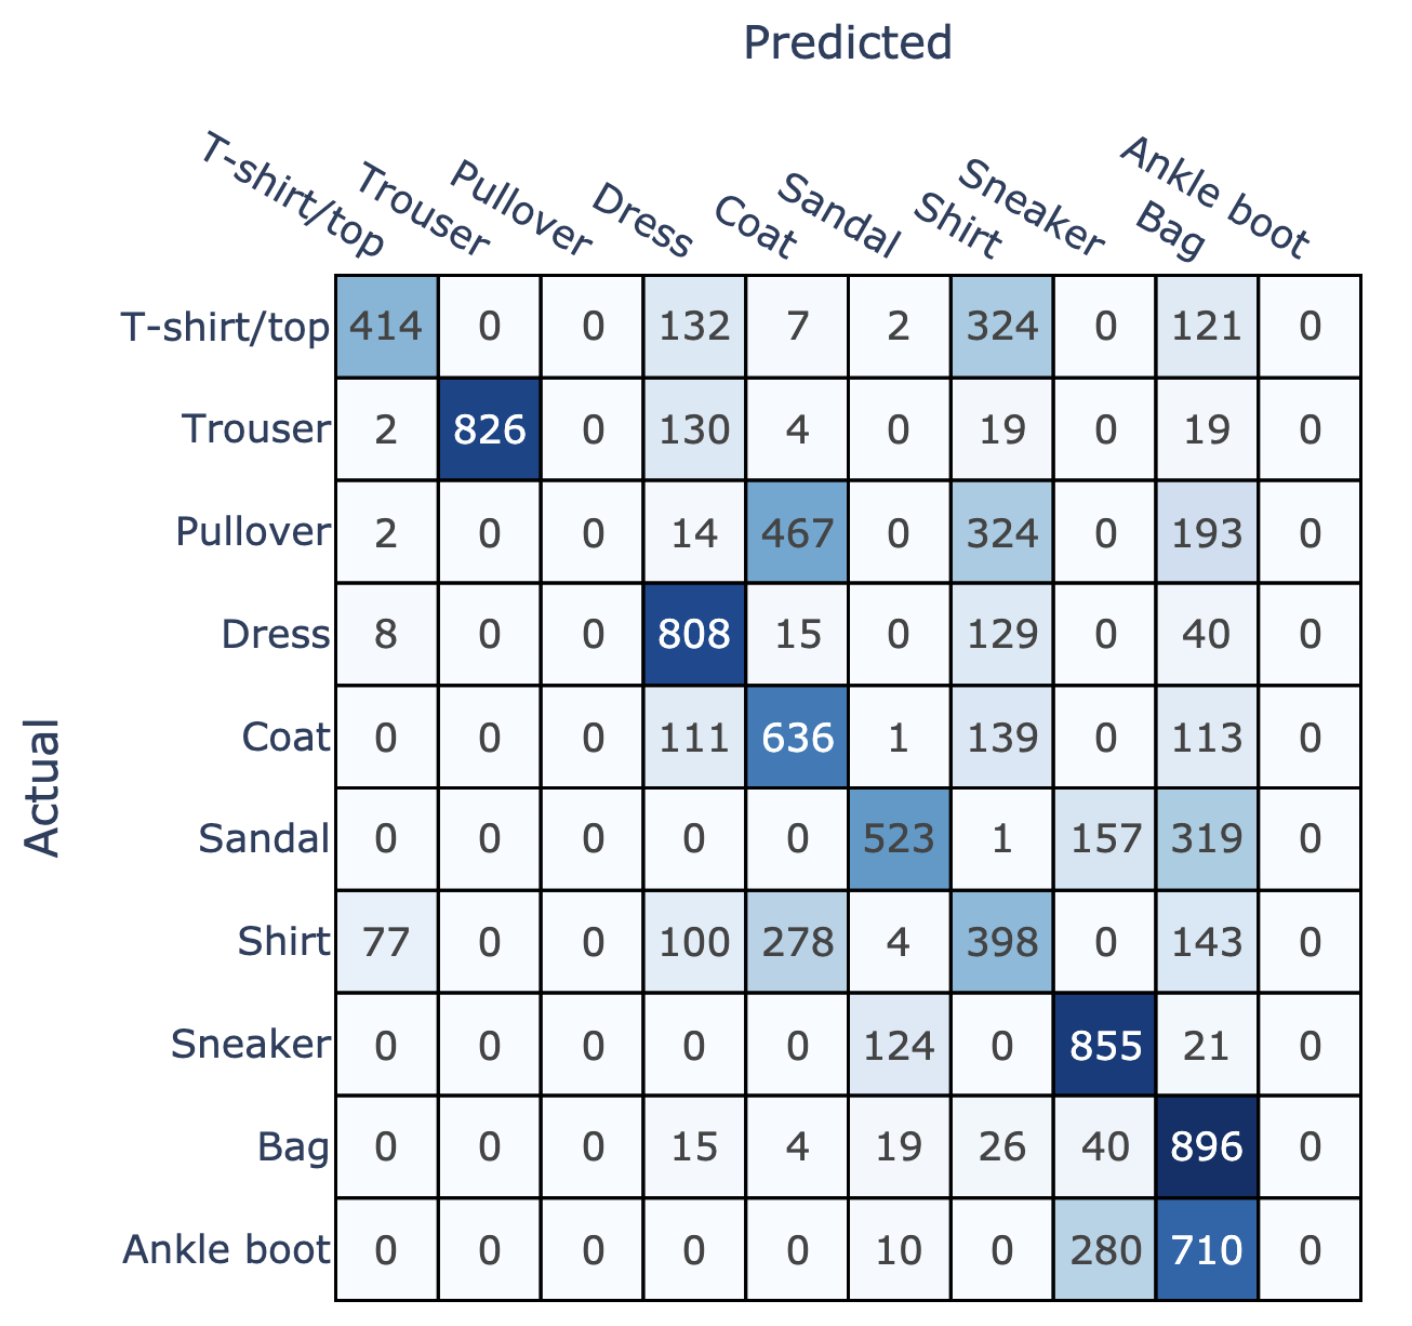
\includegraphics[width=1\linewidth]{images/CM_HybridPipeline_MajorityMapping_SVC.png}
      \subcaption{\footnotesize SVC}
    \end{minipage}\hfill
    \begin{minipage}{0.33\textwidth}
      \centering
      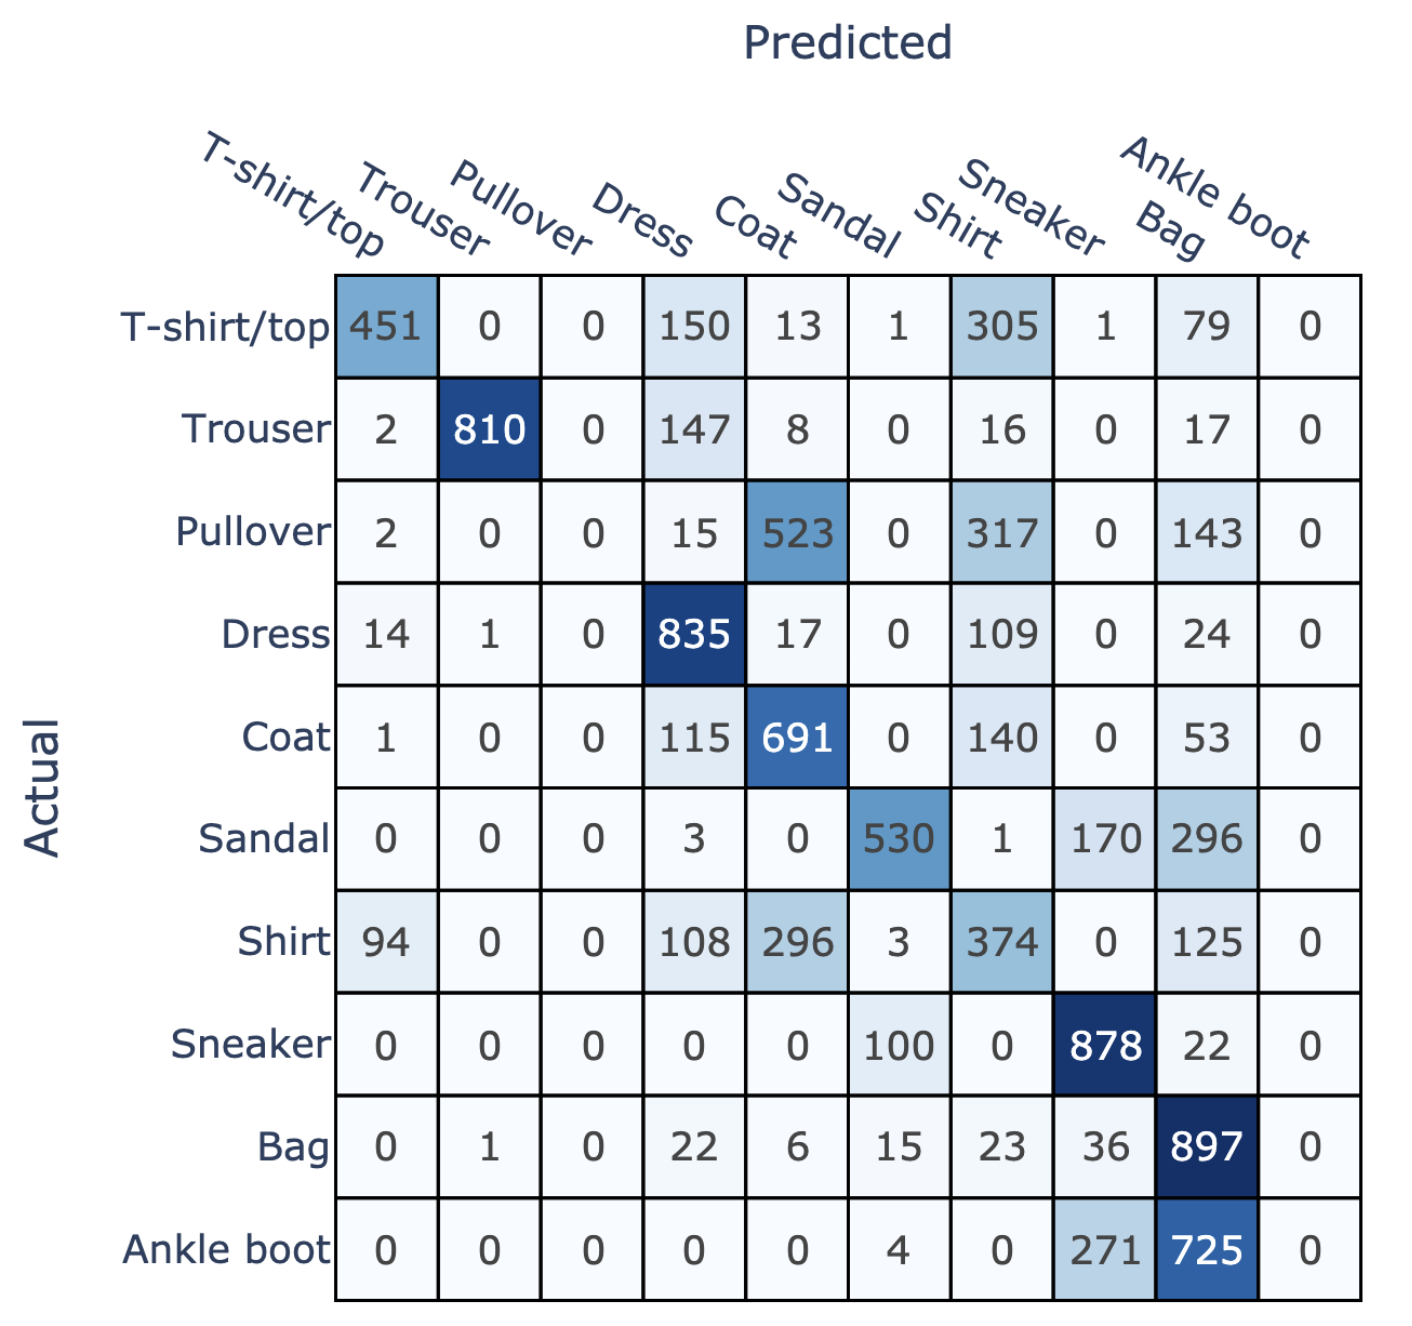
\includegraphics[width=1\linewidth]{images/CM_HybridPipeline_MajorityMapping_FCNN.png}
      \subcaption{\footnotesize FCNN}
    \end{minipage}\hfill
    \begin{minipage}{0.33\textwidth}
        \centering
        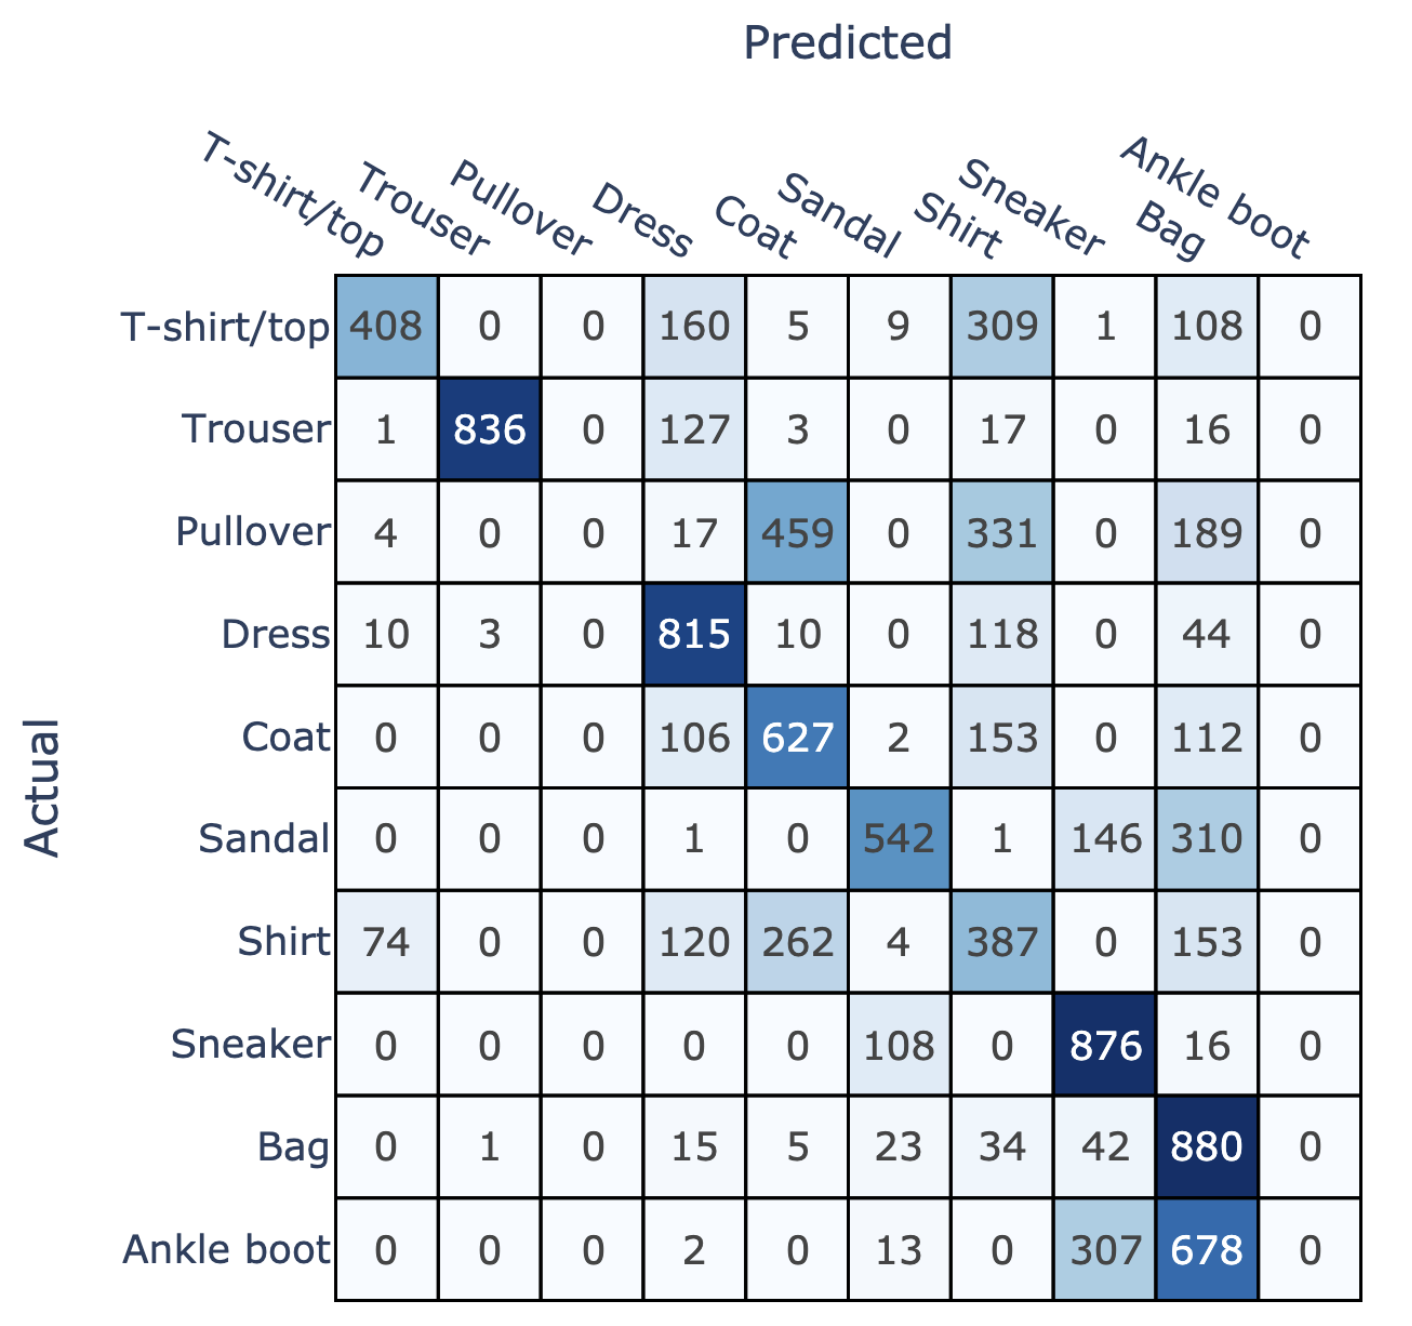
\includegraphics[width=1\linewidth]{images/CM_HybridPipeline_MajorityMapping_CNN.png}
        \subcaption{\footnotesize CNN}
    \end{minipage}
    \caption{\footnotesize Confusion matrices for classification models [Majority Mapping]}
    \label{fig:confusion_matrices_majority}
 \end{figure}

 \begin{figure}[!htb]
    \begin{minipage}{0.33\textwidth}
      \centering
      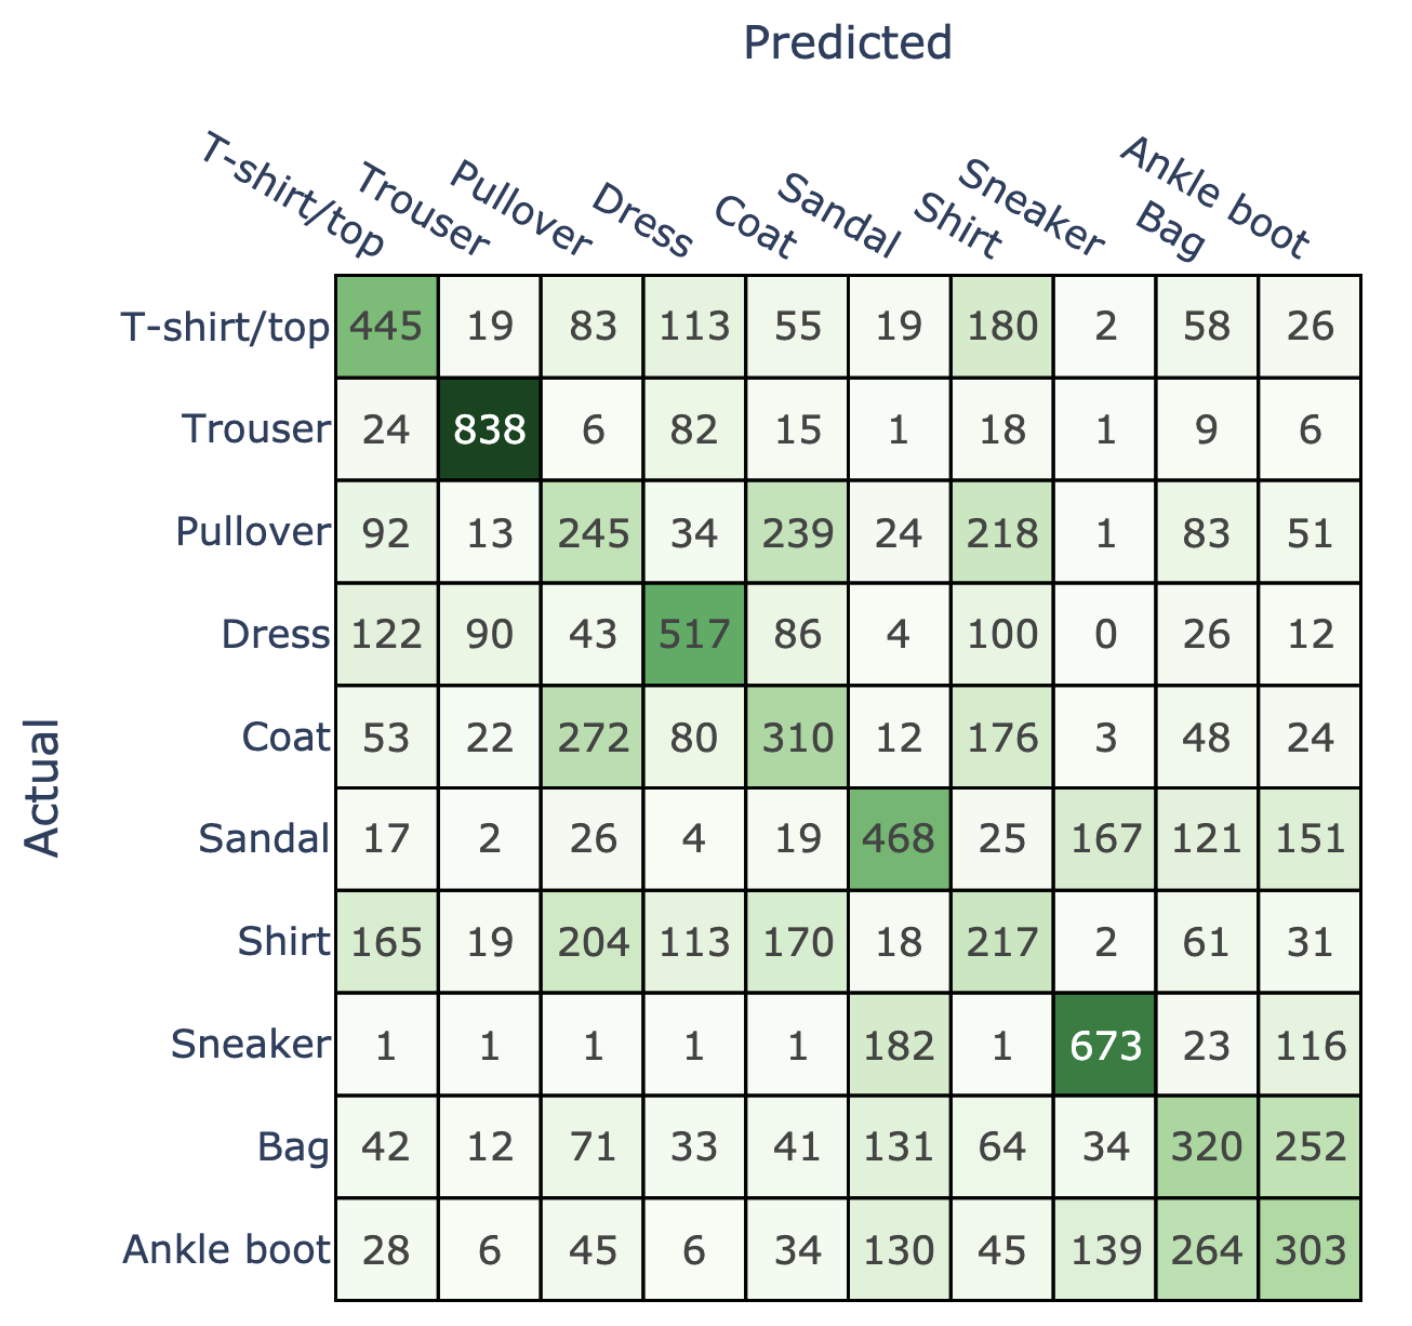
\includegraphics[width=1\linewidth]{images/CM_HybridPipeline_ProbabilisticMapping_SVC.png}
      \subcaption{\footnotesize SVC}
    \end{minipage}\hfill
    \begin{minipage}{0.33\textwidth}
      \centering
      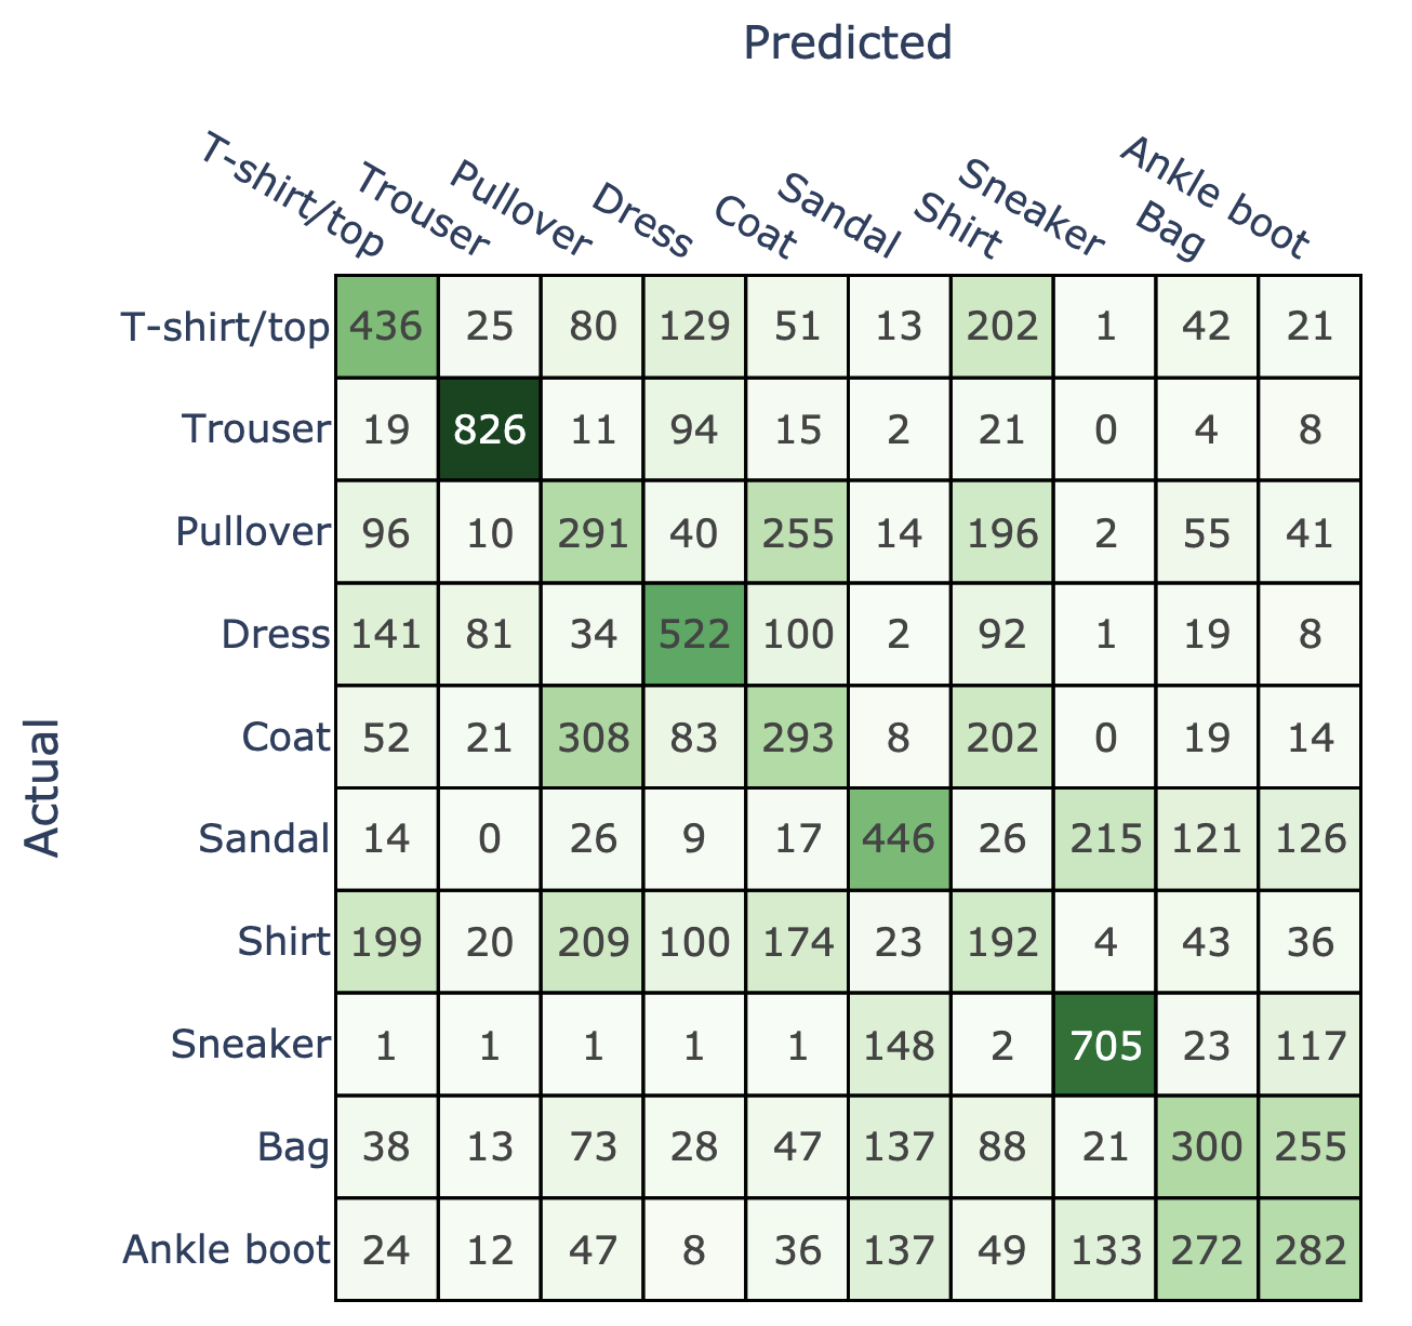
\includegraphics[width=1\linewidth]{images/CM_HybridPipeline_ProbabilisticMapping_FCNN.png}
      \subcaption{\footnotesize FCNN}
    \end{minipage}\hfill
    \begin{minipage}{0.33\textwidth}
        \centering
        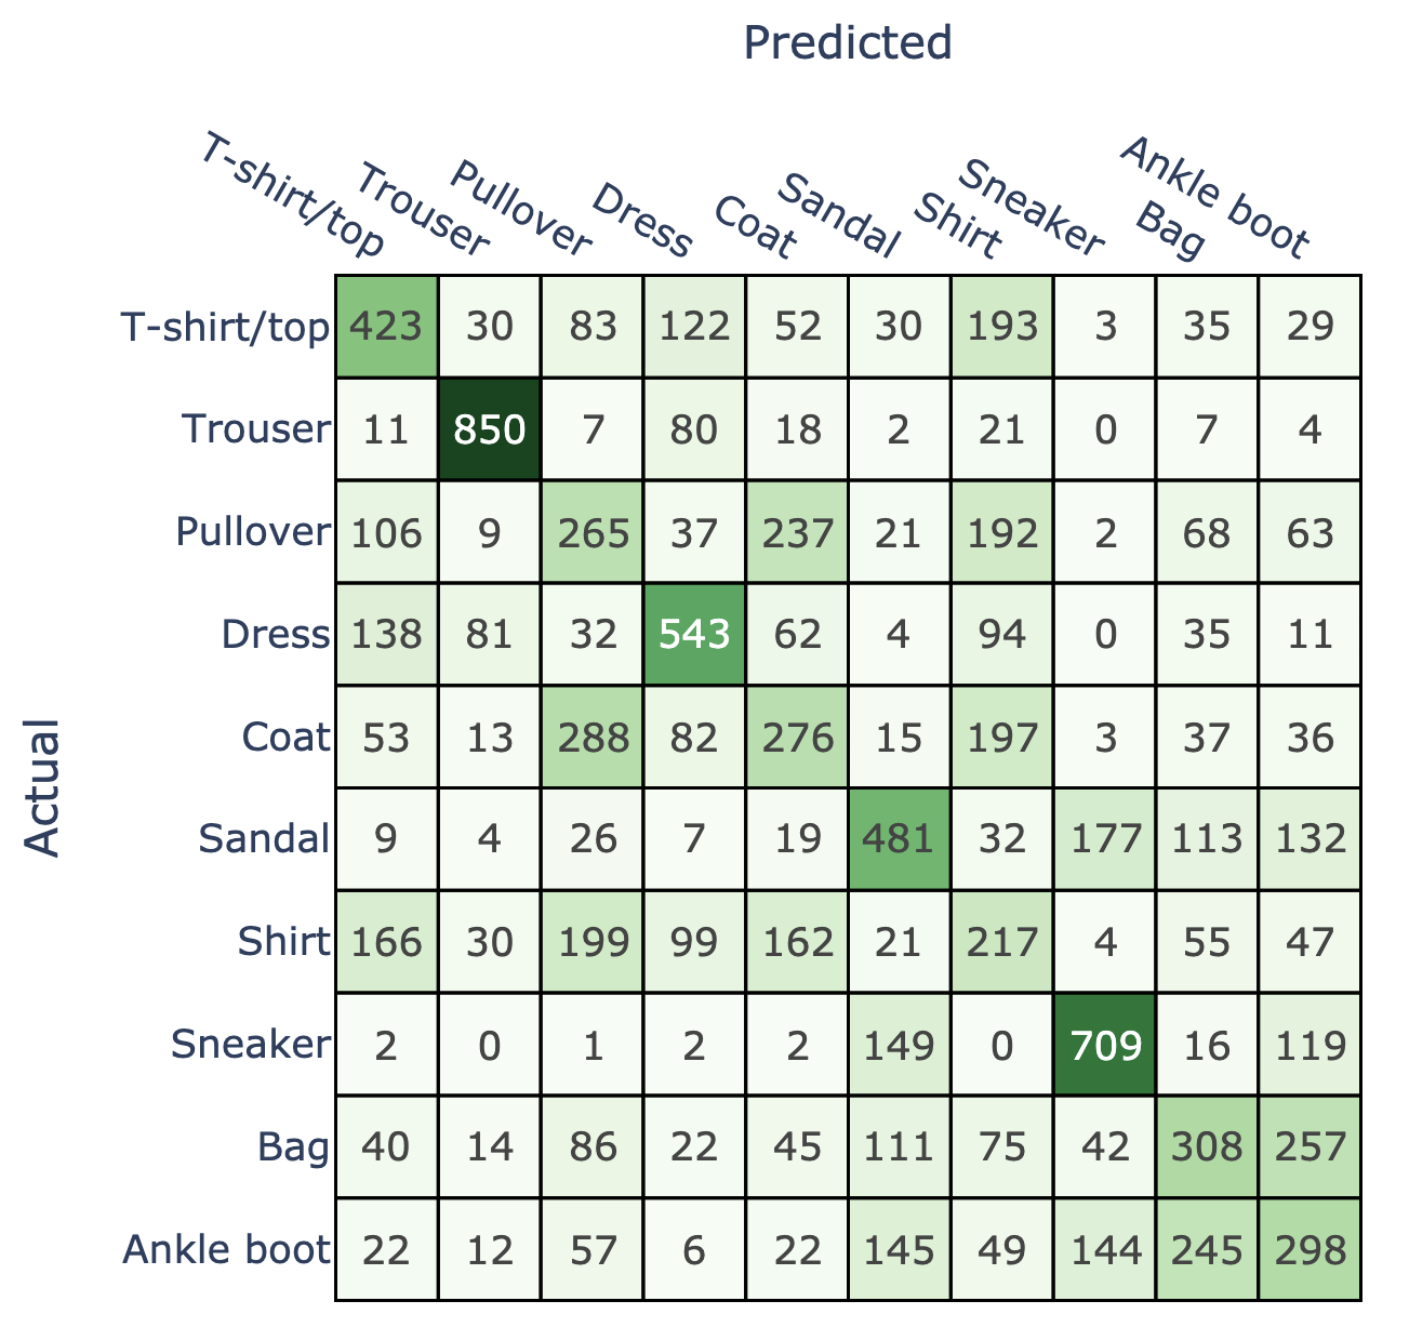
\includegraphics[width=1\linewidth]{images/CM_HybridPipeline_ProbabilisticMapping_CNN.png}
        \subcaption{\footnotesize CNN}
    \end{minipage}
    \caption{\footnotesize Confusion matrices for classification models [Probabilistic Mapping]}
    \label{fig:confusion_matrices_probabilistic}
\end{figure}

% Majority Vote Tables
\begin{table}[H]
    \centering
    \begin{minipage}{0.32\textwidth}
        \centering
        \begin{adjustbox}{max width=1\textwidth}
            \begin{tabular}{|c|c|c|c|}
                \hline
                \textbf{Class} & \textbf{Precision} & \textbf{Recall} & \textbf{F1-Score} \\ \hline
                Ankle boot & NaN & 0.00 & 0.00 \\ 
                Bag & 0.35 & 0.90 & 0.50 \\
                Coat & 0.45 & 0.64 & 0.53 \\ 
                Dress & 0.62 & 0.81 & 0.70 \\ 
                Pullover & NaN & 0.00 & 0.00 \\ 
                Sandal & 0.77 & 0.52 & 0.62 \\ 
                Shirt & 0.29 & 0.40 & 0.34 \\ 
                Sneaker & 0.64 & 0.85 & 0.73 \\ 
                T-shirt/top & 0.82 & 0.41 & 0.55 \\ 
                Trouser & 1.00 & 0.83 & 0.90 \\ \hline
            \end{tabular}
        \end{adjustbox}
        \subcaption{\footnotesize SVC}
    \end{minipage}
    \hfill
    \begin{minipage}{0.32\textwidth}
        \centering
        \begin{adjustbox}{max width=1\textwidth}
            \begin{tabular}{|c|c|c|c|}
                \hline
                \textbf{Class} & \textbf{Precision} & \textbf{Recall} & \textbf{F1-Score} \\ \hline
                Ankle boot & NaN & 0.00 & 0.00 \\ 
                Bag & 0.38 & 0.90 & 0.53 \\ 
                Coat & 0.44 & 0.69 & 0.54 \\ 
                Dress & 0.60 & 0.83 & 0.70 \\ 
                Pullover & NaN & 0.00 & 0.00 \\ 
                Sandal & 0.81 & 0.53 & 0.64 \\ 
                Shirt & 0.29 & 0.37 & 0.33 \\ 
                Sneaker & 0.65 & 0.88 & 0.75 \\ 
                T-shirt/top & 0.80 & 0.45 & 0.58 \\ 
                Trouser & 1.00 & 0.81 & 0.89 \\ \hline
            \end{tabular}
        \end{adjustbox}
        \subcaption{\footnotesize FCNN}
    \end{minipage}
    \hfill
    \begin{minipage}{0.32\textwidth}
        \centering
        \begin{adjustbox}{max width=1\textwidth}
            \begin{tabular}{|c|c|c|c|}
                \hline
                \textbf{Class} & \textbf{Precision} & \textbf{Recall} & \textbf{F1-Score} \\ \hline
                Ankle boot & NaN & 0.00 & 0.00 \\ 
                Bag & 0.35 & 0.88 & 0.50 \\ 
                Coat & 0.46 & 0.63 & 0.53 \\ 
                Dress & 0.60 & 0.81 & 0.69 \\ 
                Pullover & NaN & 0.00 & 0.00 \\ 
                Sandal & 0.77 & 0.54 & 0.64 \\ 
                Shirt & 0.29 & 0.39 & 0.33 \\ 
                Sneaker & 0.64 & 0.88 & 0.74 \\ 
                T-shirt/top & 0.82 & 0.41 & 0.55 \\ 
                Trouser & 1.00 & 0.84 & 0.91 \\ \hline
            \end{tabular}
        \end{adjustbox}
        \subcaption{\footnotesize CNN}
    \end{minipage}
    \caption{\footnotesize Classification reports for models [Majority Mapping]}
    \label{tab:ClassificationReport_Majority}
\end{table}

% Proportional Vote Tables
\begin{table}[H]
    \centering
    \begin{minipage}{0.32\textwidth}
        \centering
        \begin{adjustbox}{max width=1\textwidth}
            \begin{tabular}{|c|c|c|c|}
                \hline
                \textbf{Class} & \textbf{Precision} & \textbf{Recall} & \textbf{F1-Score} \\ \hline
                Ankle boot & 0.31 & 0.30 & 0.31 \\ 
                Bag & 0.32 & 0.32 & 0.32 \\ 
                Coat & 0.32 & 0.31 & 0.31 \\ 
                Dress & 0.53 & 0.52 & 0.52 \\ 
                Pullover & 0.25 & 0.24 & 0.25 \\ 
                Sandal & 0.47 & 0.47 & 0.47 \\ 
                Shirt & 0.21 & 0.22 & 0.21 \\ 
                Sneaker & 0.66 & 0.67 & 0.67 \\ 
                T-shirt/top & 0.45 & 0.45 & 0.45 \\ 
                Trouser & 0.82 & 0.84 & 0.83 \\ \hline
            \end{tabular}
        \end{adjustbox}
        \subcaption{\footnotesize SVC}
    \end{minipage}
    \hfill
    \begin{minipage}{0.32\textwidth}
        \centering
        \begin{adjustbox}{max width=1\textwidth}
            \begin{tabular}{|c|c|c|c|}
            \hline
            \textbf{Class} & \textbf{Precision} & \textbf{Recall} & \textbf{F1-Score} \\ \hline
            Ankle boot & 0.31 & 0.28 & 0.30 \\ 
            Bag & 0.33 & 0.30 & 0.32 \\ 
            Coat & 0.30 & 0.29 & 0.29 \\ 
            Dress & 0.51 & 0.52 & 0.52 \\ 
            Pullover & 0.27 & 0.29 & 0.28 \\ 
            Sandal & 0.48 & 0.45 & 0.46 \\ 
            Shirt & 0.18 & 0.19 & 0.19 \\ 
            Sneaker & 0.65 & 0.70 & 0.68 \\ 
            T-shirt/top & 0.43 & 0.44 & 0.43 \\ 
            Trouser & 0.82 & 0.83 & 0.82 \\ \hline
            \end{tabular}
        \end{adjustbox}
        \subcaption{\footnotesize FCNN}
    \end{minipage}
    \hfill
    \begin{minipage}{0.32\textwidth}
        \centering
        \begin{adjustbox}{max width=1\textwidth}
            \begin{tabular}{|c|c|c|c|}
                \hline
                \textbf{Class} & \textbf{Precision} & \textbf{Recall} & \textbf{F1-Score} \\ \hline
                Ankle boot & 0.30 & 0.30 & 0.30 \\ 
                Bag & 0.34 & 0.31 & 0.32 \\ 
                Coat & 0.31 & 0.28 & 0.29 \\ 
                Dress & 0.54 & 0.54 & 0.54 \\ 
                Pullover & 0.25 & 0.27 & 0.26 \\ 
                Sandal & 0.49 & 0.48 & 0.49 \\ 
                Shirt & 0.20 & 0.22 & 0.21 \\ 
                Sneaker & 0.65 & 0.71 & 0.68 \\ 
                T-shirt/top & 0.44 & 0.42 & 0.43 \\ 
                Trouser & 0.81 & 0.85 & 0.83 \\ \hline
            \end{tabular}
        \end{adjustbox}
        \subcaption{\footnotesize FCNN}
    \end{minipage}
    \caption{\footnotesize Classification reports for models [Probabilistic Mapping]}
    \label{tab:ClassificationReport_Probabilistic}
\end{table}

When adopting the majority labeling approach, we observe NaN values in the precision metric for certain classes. 
This issue arises because the precision computation involves dividing by the total number of predictions for a class, 
and some clothing items are never predicted. Specifically, this affects the ankle boot and pullover classes, which 
consequently exhibit zero recall and F1-scores across all three models (\emph{SVC, FCNN, CNN}). This limitation is mitigated 
by adopting the probabilistic mapping approach, where no class is entirely ignored. While this eliminates NaN values 
and zero metrics, class-level performance does not generally improve. This outcome was expected, since the probabilistic 
approach accounts for minor class contributions within a cluster, which can reduce the overall representativeness of the 
dominant labels. To further analyze this, I retrieved the balanced accuracy from the confusion matrices for both labeling approaches. 
Under the majority mapping approach, the balanced accuracy values resulted 0.54 (\emph{SVC}), 0.55 (\emph{FCNN}) and 0.54 (\emph{CNN}), reflecting modest 
but consistent performance across the models. In contrast, with the probabilistic mapping approach, balanced accuracies decrease
to 0.43 (\emph{SVC}), 0.43 (\emph{FCNN}) and 0.44 (\emph{CNN}).\\[0.2cm]
Among the categories, trousers consistently emerge as the best-classified item across all models and approaches. Remarkably, under the 
majority labeling approach, all models achieve a precision of 1.0 for trousers, meaning that every predicted trouser was correct. This 
result reflects the distinct geometric separation of trousers in the data. Other relatively well-classified categories include T-shirts/tops, 
sandals, and sneakers, with the latter two indicating the models' ability to effectively capture footwear patterns. In contrast, ankle boots 
exhibit poor classification metrics, driven by significant overlap with other classes. Similarly, bags also perform poorly, 
likely due to their observed overlap with ankle boots. Finally, shirts emerge as the most challenging category to classify across all 
models and approaches, with the models consistently struggling to distinguish shirts.\\[0.2cm]
These results, combined with the findings from \Cref{hybrid_model_tuning}, allow us to draw some important conclusions about the 
hybrid pipeline we built. My opinion is that the pipeline effectively captured features and patterns from the unlabeled data during 
the clustering phase. In fact, all the models outperform both the random guessing and the dummy classifier (given the balanced nature 
of the training and test sets, these two almost coincide), which would achieve approximately a 10\% of accuracy. However, there is a notable drop
in performance when transitioning from cluster IDs predictions to the original Fashion-MNIST labels. This is reflected by the 
models’ difficulty in distinguishing between certain categories, which was already clear during the clustering phase 
(recall \Cref{fig:cluster_composition}), where these classes were often overlapped and grouped together. 
The relatively low accuracies (43-44\%) achieved in our mapping step are in contrast to the results typically obtained 
with fully supervised learning on Fashion-MNIST, as we'll see in \Cref{fully_supervised_approach}. These results underscore the inherent 
challenges of our unsupervised-to-supervised approach: while the pipeline demonstrates its ability to learn structure from unlabeled data, 
the limitations in accurately mapping clusters to fine-grained categories highlight the complexity of the task, particularly in cases 
of significant class overlapping.
\newpage
    \section{Fully Supervised Approach}\label{fully_supervised_approach}
In this last section we follow the same steps of \Cref{hybrid_model_tuning,hybrid_pipeline_evaluation}, referring now
to the true labels from the dataset. Again, I relied on a 5-fold cross validation in order to tune different configurations for each model,
comparing the performance in terms of both balanced accuracy and computational cost. Since the hyperparamter grids were the same as the 
ones used in the previous section, I will report directly the best configurations:
\begin{itemize}
    \item \textbf{SVC}: gaussian kernel, with gamma=0.01 and C=10;
    \item \textbf{FCNN}: 512 hidden units, ReLU non linearity and dropout rate of 0.5, trained with 
    a learning rate of 0.01 and a batch size of 256;
    \item \textbf{CNN}:  ReLU non linearity, AvgPool2d pooling and batch normalization, trained with
    a learning rate of 0.01 and a batch size of 64.
\end{itemize}
Results from cross validation are summarized in \Cref{tab:model_comparison_FullySupervised}, 
while the performance on the test set is presented in \Cref{fig:confusion_matrices_FullySupervised,tab:ClassificationReport_FullySupervised}.

\begin{table}[h!]
    \centering
    \begin{adjustbox}{max width=0.85\textwidth}
    \begin{tabular}{|l|c|c|c|}
    \hline
    \textbf{Model} & \textbf{Balanced Accuracy} & \textbf{Training Time (s)} & \textbf{Inference Time (s)}  \\
    \hline
    SVC & 0.8656  $\pm$ 0.0070 & 1.5808 $\pm$ 0.0108 & 1.1168 $\pm$ 0.0046 \\
    FCNN & 0.8424 $\pm$ 0.0046 & 2.5826 $\pm$ 0.1118 & 0.0107 $\pm$ 0.0034 \\
    CNN & 0.8158  $\pm$ 0.0085 & 5.4935 $\pm$ 0.0034 & 0.0497 $\pm$ 0.0000 \\
    \hline
    \end{tabular}
    \end{adjustbox}
    \caption{\footnotesize Comparison of SVC, FCNN, and CNN in terms of balanced accuracy, training time, and inference time. 
    All the values are expressed as confidence intervals at 95\% level.}
    \label{tab:model_comparison_FullySupervised}
\end{table}

\begin{figure}[!htb]
    \begin{minipage}{0.33\textwidth}
      \centering
      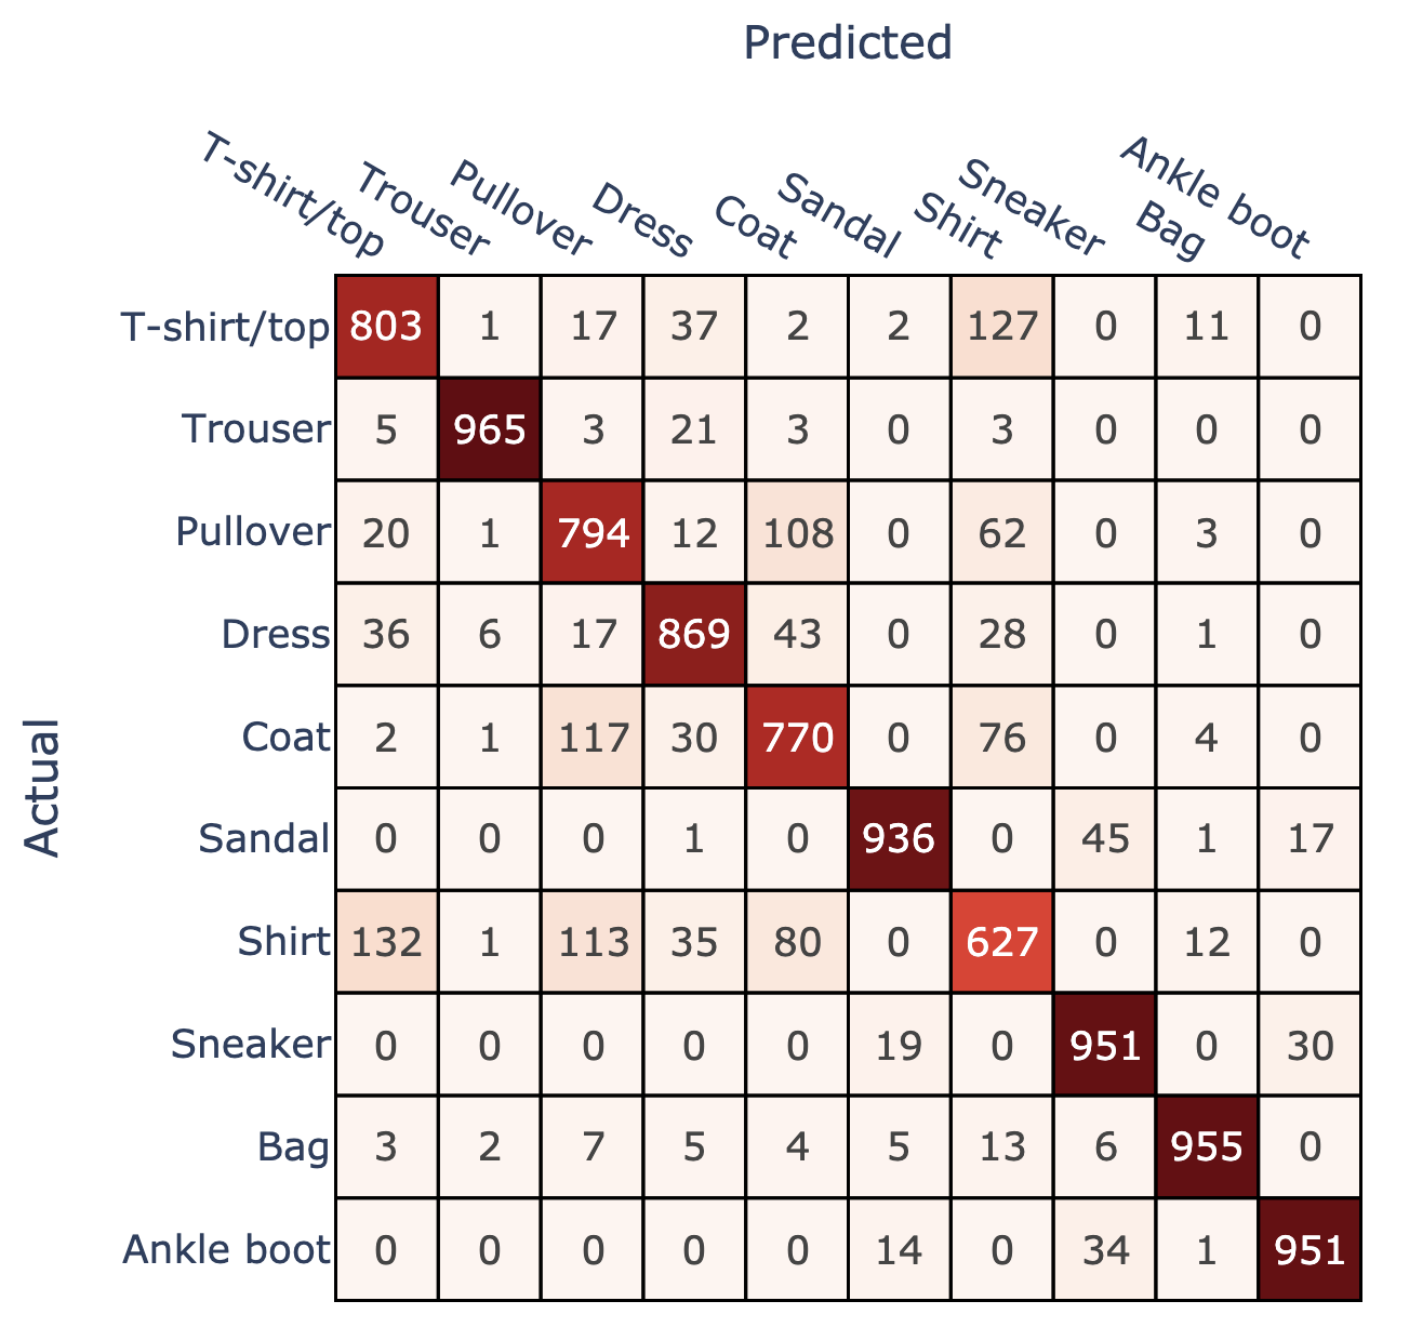
\includegraphics[width=1\linewidth]{images/CM_FullySupervised_SVC.png}
      \subcaption{\footnotesize SVC}
    \end{minipage}\hfill
    \begin{minipage}{0.33\textwidth}
      \centering
      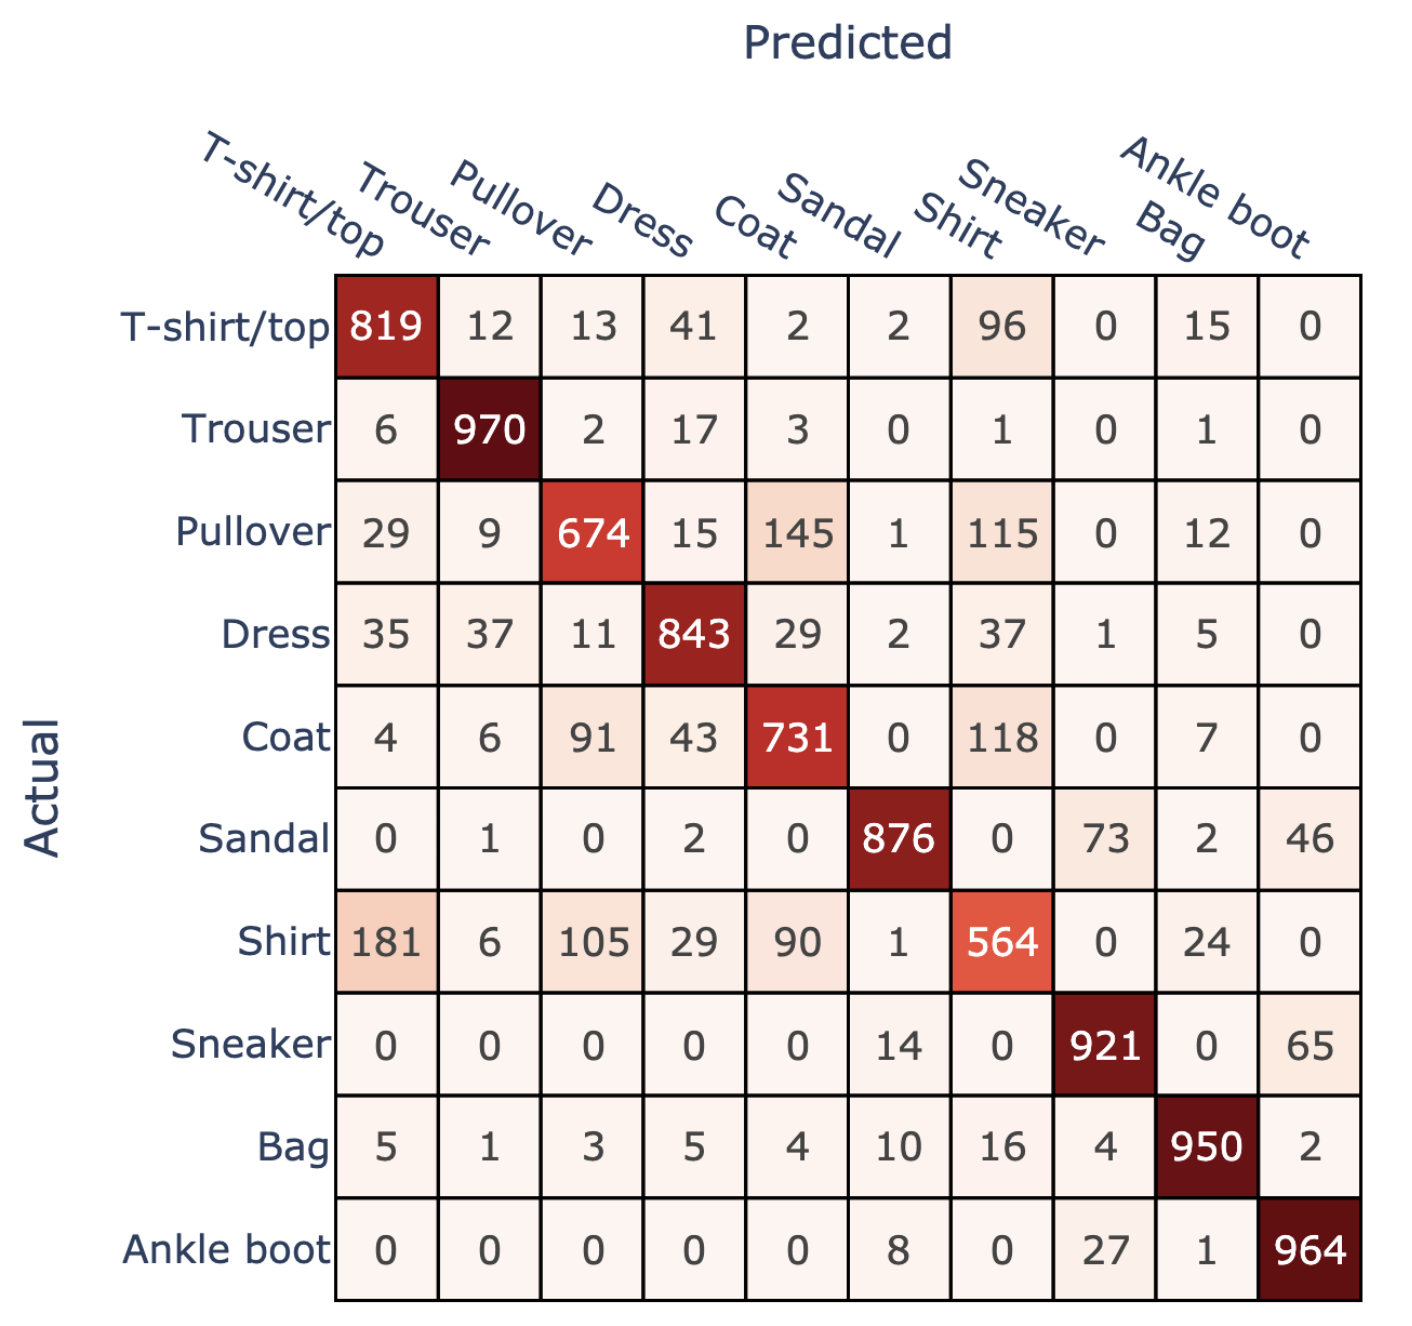
\includegraphics[width=1\linewidth]{images/CM_FullySupervised_FCNN.png}
      \subcaption{\footnotesize FCNN}
    \end{minipage}\hfill
    \begin{minipage}{0.33\textwidth}
        \centering
        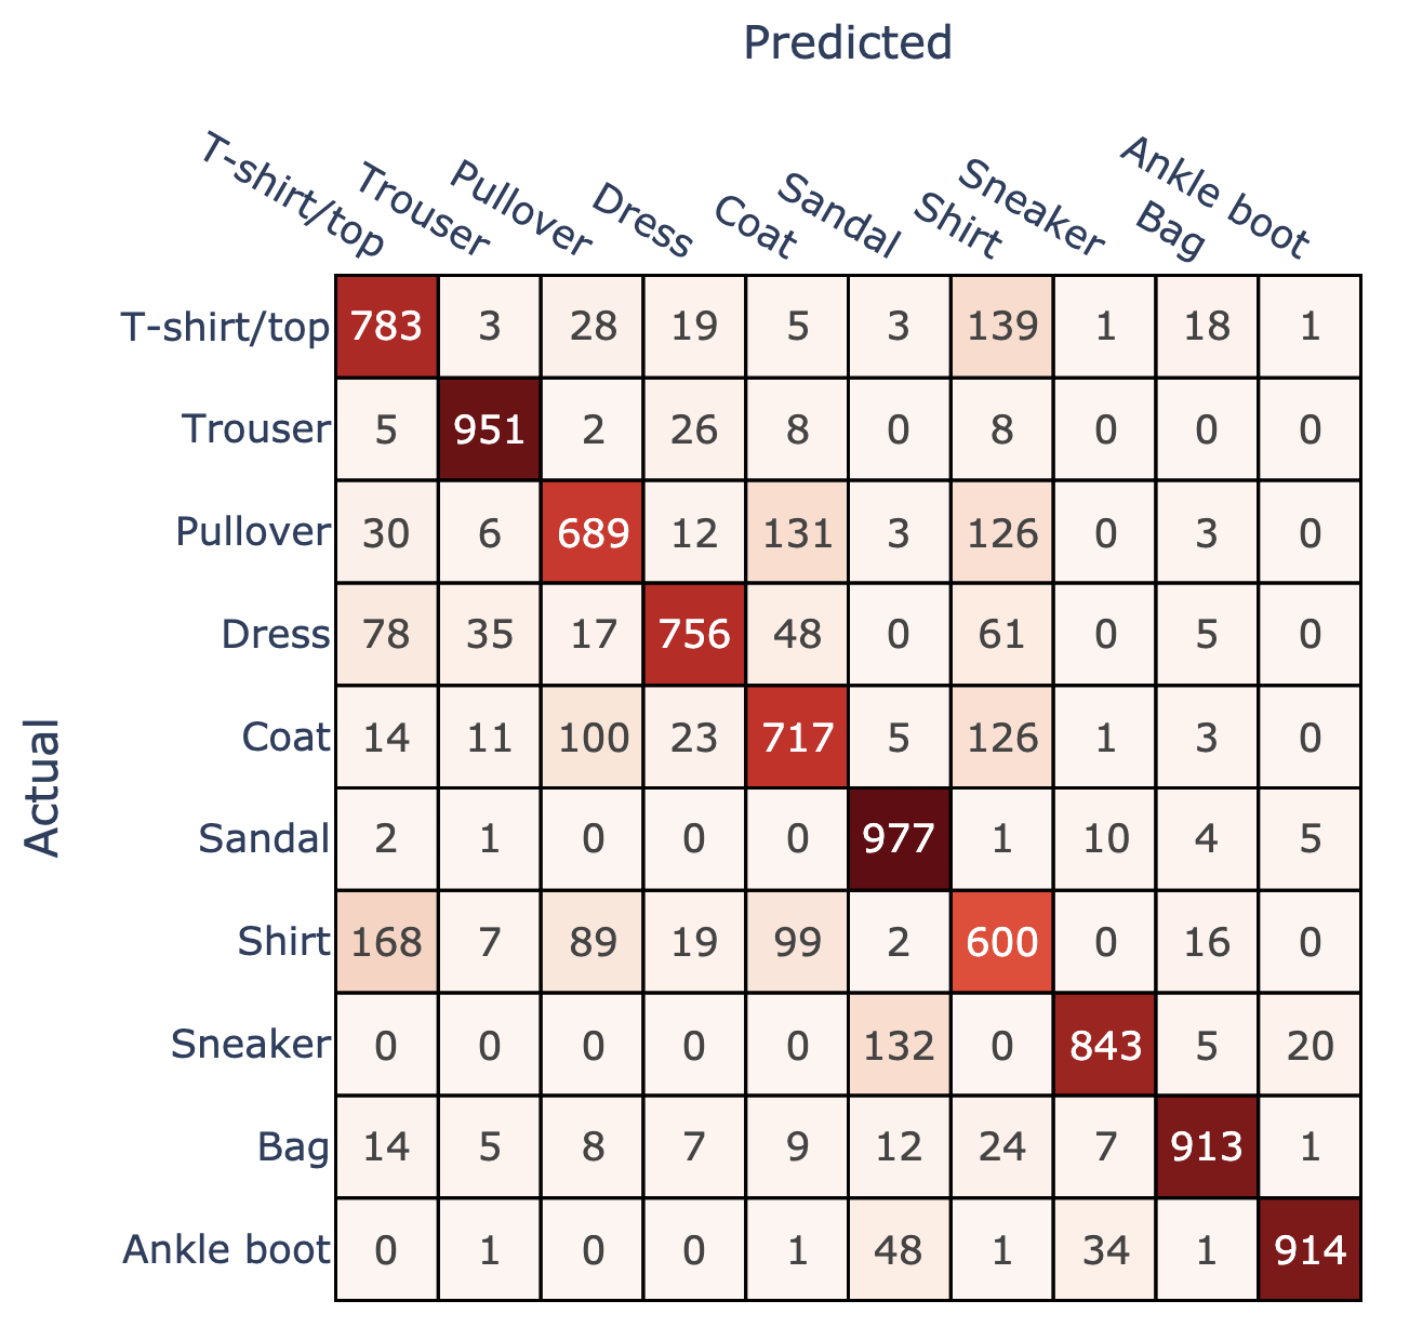
\includegraphics[width=1\linewidth]{images/CM_FullySupervised_CNN.png}
        \subcaption{\footnotesize CNN}
    \end{minipage}
    \caption{\footnotesize Confusion matrices for classification models [Fully Supervised Approach]}
    \label{fig:confusion_matrices_FullySupervised}
 \end{figure}


 \begin{table}[H]
    \centering
    \begin{minipage}{0.32\textwidth}
        \centering
        \begin{adjustbox}{max width=1\textwidth}
            \begin{tabular}{|c|c|c|c|}
                \hline
                \textbf{Class}     & \textbf{Precision} & \textbf{Recall} & \textbf{F1-Score} \\ \hline
                Ankle boot         & 0.95               & 0.95            & 0.95              \\
                Bag                & 0.97               & 0.95            & 0.96              \\
                Coat               & 0.76               & 0.77            & 0.77              \\
                Dress              & 0.86               & 0.87            & 0.86              \\
                Pullover           & 0.74               & 0.79            & 0.77              \\
                Sandal             & 0.96               & 0.94            & 0.95              \\
                Shirt              & 0.67               & 0.63            & 0.65              \\
                Sneaker            & 0.92               & 0.95            & 0.93              \\
                T-shirt/top        & 0.80               & 0.80            & 0.80              \\
                Trouser            & 0.99               & 0.96            & 0.98              \\ \hline
            \end{tabular}
        \end{adjustbox}
        \subcaption{\footnotesize SVC}
    \end{minipage}
    \hfill
    \begin{minipage}{0.32\textwidth}
        \centering
        \begin{adjustbox}{max width=1\textwidth}
            \begin{tabular}{|c|c|c|c|}
                \hline
                \textbf{Class}     & \textbf{Precision} & \textbf{Recall} & \textbf{F1-Score} \\ \hline
                Ankle boot         & 0.90               & 0.96            & 0.93              \\
                Bag                & 0.93               & 0.95            & 0.94              \\
                Coat               & 0.73               & 0.73            & 0.73              \\
                Dress              & 0.85               & 0.84            & 0.85              \\
                Pullover           & 0.75               & 0.67            & 0.71              \\
                Sandal             & 0.96               & 0.88            & 0.92              \\
                Shirt              & 0.60               & 0.56            & 0.58              \\
                Sneaker            & 0.90               & 0.92            & 0.91              \\
                T-shirt/top        & 0.76               & 0.82            & 0.79              \\
                Trouser            & 0.93               & 0.97            & 0.95              \\ \hline
            \end{tabular}
        \end{adjustbox}
        \subcaption{\footnotesize FCNN}
    \end{minipage}
    \hfill
    \begin{minipage}{0.32\textwidth}
        \centering
        \begin{adjustbox}{max width=1\textwidth}
            \begin{tabular}{|c|c|c|c|}
                \hline
                \textbf{Class}     & \textbf{Precision} & \textbf{Recall} & \textbf{F1-Score} \\ \hline
                Ankle boot         & 0.97               & 0.91            & 0.94              \\
                Bag                & 0.94               & 0.91            & 0.93              \\
                Coat               & 0.70               & 0.72            & 0.71              \\
                Dress              & 0.88               & 0.76            & 0.81              \\
                Pullover           & 0.74               & 0.69            & 0.71              \\
                Sandal             & 0.83               & 0.98            & 0.90              \\
                Shirt              & 0.55               & 0.60            & 0.58              \\
                Sneaker            & 0.94               & 0.84            & 0.89              \\
                T-shirt/top        & 0.72               & 0.78            & 0.75              \\
                Trouser            & 0.93               & 0.95            & 0.94              \\ \hline
            \end{tabular}
        \end{adjustbox}
        \subcaption{\footnotesize CNN}
    \end{minipage}
    \caption{\footnotesize Classification reports for models [Fully Supervised Approach]}
    \label{tab:ClassificationReport_FullySupervised}
\end{table}

The models trained with the fully supervised approach exhibit significantly higher performance across all metrics if compared 
to their counterparts with ID-mapped labels. From a global perspective, the overall balanced accuracy of \emph{SVC}, \emph{FCNN} and \emph{CNN} 
increased to 0.86, 0.83, and 0.82, respectively. A notable improvement is also observed at a class level, where the values 
of precision, recall, and F1-score are generally higher than those obtained with the hybrid pipeline. This result is not 
particularly surprising and, in my opinion, can be attributed to two main factors. First, in the fully supervised approach, 
we fed the model with 728-pixel images, which inherently carry far more information than the 10-dimensional vectors used at the very 
beginning of the hybrid pipeline. The higher dimensionality allows the models to capture richer and more detailed patterns, significantly 
contributing to their superior performance. Second, the fully supervised approach involves training the models directly 
on the data, whereas the hybrid pipeline involves multiple stages, each introducing potential sources of error. During the 
dimensionality reduction phase, significant information loss occurs, as highlighted by the spectrum in \Cref{fig:kpa_spectrum}
and by the estimation of the manifold's intrinsic dimensionality. 
In the clustering phase, errors may occur if the algorithm fails to accurately represent the underlying structure of the data.
Besides the proposed dimensionality reduction method, I experimented with more advanced techniques such as t-SNE and UMAP, but 
these did not yield any significant improvement. My last trial was an AutoEncoder architecture, in order to leverage the 
encoder component to reduce data dimensionality. Although this approach made the cluster separation more distinct, 
it did not enhance classification performance. Finally, the mapping stage adds another layer of complexity, where issues can emerge from 
both the majority and the probabilistic mapping. These accumulated imperfections likely explain the performance gap between the 
two methods.\\[0.2cm]
From a qualitative perspective, trousers, ankle boots, sneakers, sandals, and dresses are consistently the best-classified labels. 
While the performance for other labels has improved, the models still struggle to correctly classify items such as shirts, coats, 
and pullovers. This observation aligns with the ones drawn in previous sections, proving our
pipeline to be valuable at least in gaining preliminary insights into the data structure.\\[0.2cm]
Interestingly, as in the hybrid approach, the model with the best performance is \emph{SVC}. This outcome surprised me a lot, 
as in the fully supervised setting, the model learns directly from the original images rather than from projections 
obtained through kernel-based dimensionality reduction. This suggests that the kernel trick applied to \emph{Fashion-MNIST} dataset may 
be particularly effective in mapping data points into a favorable feature space. However, it is crucial to point out that our 
analysis relied on a reduced slice of the dataset. If we were to train on the entire dataset, neural networks would significantly 
outperform \emph{SVC}, due to their ability to handle large datasets efficiently and effectively.




\end{document}
